\documentclass[final,11pt]{article}
%
\usepackage[left=1in, top=1in, bottom=1in, right=1in]{geometry}
\usepackage{enumitem}


% packages 
\usepackage{latexsym,amssymb,amsmath,amsthm,color}
%\usepackage{theorem}
\usepackage{graphicx}
\usepackage[colorlinks=true]{hyperref}
\hypersetup{urlcolor=blue, citecolor=red}
%\usepackage{algorithmic}
%\usepackage{algorithm}
\usepackage{cite}
\usepackage[table]{xcolor}



% -------------- macros
\newcommand{\p}{\partial}
\def\Cb{\overline{C}}
\newcommand{\R}{\mathbb{R}}
\newcommand{\N}{\mathbb{N}}
\newcommand{\cov}{\mathrm{cov}}
\newcommand{\iid}{\stackrel{iid}{\sim}}
\newcommand{\F}{\mathcal{F}}%
\newcommand{\be}{\begin{equation}}
\newcommand{\ee}{\end{equation}}
\newcommand{\bea}{\begin{eqnarray}}
\newcommand{\eea}{\end{eqnarray}}
\newcommand{\rebut}[1]{{\color{blue}{#1}}}
%\newcommand{\p}{\partial}
\newcommand{\ttt}{\tilde}
\newcommand{\E}[1]{\mathrm{E}\left\{{#1} \right\}}
\newcommand{\Ez}[1]{\mathrm{E}_z\left\{{#1} \right\}}
\newcommand{\mat}[1]{\mathbf{{#1}}}
\newcommand{\trace}{\mathrm{trace}}
\newtheorem{theorem}{Theorem}[section]
\newtheorem{lemma}{Lemma}[section]
\newtheorem{proposition}{Proposition}[section]
\newtheorem{remark}{Remark}[section]
\newcommand*{\skipnumber}[2][1]{%
   {\renewcommand*{\alglinenumber}[1]{}\State #2}%
   \addtocounter{ALG@line}{-#1}}
%
\def\Wb{\overline{W}}
\def\td{\tilde \delta}
\def\tL{\tilde L}
\def\tU{\tilde U}
\def\tt{\tilde t}
\def\Vector#1{\mbox{\boldmath $#1$}}
\def\vH{{\Vector H}}
\def\vx{{\Vector x}}
\def\vy{{\Vector y}}
\def\vz{{\Vector z}}
\def\vj{{\Vector j}}
\def\vk{{\Vector k}}
\def\vt{{\Vector t}}
\def\ve{{\Vector e}}
\def\vb{{\Vector b}}
\def\vg{{\Vector g}}
\def\vn{{\Vector n}}
\def\vp{{\Vector p}}
\def\vr{{\Vector r}}
\def\vS{{\Vector S}}
\def\vV{{\Vector V}}
\def\vY{{\Vector Y}}
\def\vX{{\Vector X}}
\def\vv{{\Vector v}}
\def\vu{{\Vector u}}
\def\vQ{{\Vector Q}}
\def\vZ{{\Vector Z}}
\def\vN{{\Vector N}}
\def\vF{{\Vector F}}
\def\vC{{\Vector C}}
\def\vq{{\Vector q}}
\def\vom{{\Vector \omega}}
\def\vtau{{\Vector \tau}}
\def\F{{\rm\bf F}}
\def\sech{{\rm sech}}
\def\funnyzeta{\varsigma}
\def\tQ{\stackrel{\ldots}{Q}}
%
\def\Re{{\rm Re}}
\def\Sc{{\rm Sc}}
\def\Pe{{\rm Pe}}
\def\Pr{{\rm Pr}}
\def\Da{{\rm Da}}
\def\rf{{\rm ref}}
\def\eps{{\varepsilon}}
\def\ep{\epsilon'}
\def\O{{\rm O}}
\def\1{{\rm 1}}
\def\so{^{\rm (0)}}
\def\s1{^{\rm (1)}}
\def\d{{\rm d}}
\def\ttm{^{{\rm ttm}}}
\def\img{^{\rm im}}
\def\si{^{\rm si}}
%
\def\ol{\overline}
%
\def\tn{^{n}}
\def\tnm{^{n-1}}
\def\new#1{{\bf #1}}
%\def\new#1{{#1}}

\renewcommand{\L}{\mathcal{L}}
\newcommand{\Q}{\mathcal{Q}}
\newcommand{\U}{\mathcal{U}}
\newcommand{\G}{\mathcal{N}}
\newcommand{\V}{\mathbb{V}}
\renewcommand{\P}{\mathrm{P}}
\newcommand{\B}{\mathcal{B}}
\renewcommand{\vec}[1]{{\mathchoice
                     {\mbox{\boldmath$\displaystyle{#1}$}}
                     {\mbox{\boldmath$\textstyle{#1}$}}
                     {\mbox{\boldmath$\scriptstyle{#1}$}}
                     {\mbox{\boldmath$\scriptscriptstyle{#1}$}}}}
\newcommand{\var}[1]{{\mathrm{Var}}\left( {#1} \right)}
\newcommand{\normim}[1]{\left\| {#1} \right\|_{\scriptscriptstyle L^{2}(\Omega^{*})}}
\newcommand{\avemu}[1]{\mathrm{E}\left({#1}\right)}
\newcommand{\ave}[1]{\left\langle {#1} \right\rangle}
\newcommand{\prob}[1]{\mathrm{Prob}\left\{ {#1} \right\}}
\newcommand{\ind}[1]{\mathrm{\chi}_{\scriptscriptstyle {#1} }}
\newcommand{\NISP}{\mathcal{S}}
\newcommand{\xxi}{\vec{\xi}}
\newcommand{\ip}[2]{\left\langle {#1}, {#2} \right\rangle}
\newcommand{\ipmu}[2]{\left( {#1}, {#2} \right)_\mu}
\newcommand{\norm}[1]{\left\| {#1} \right\|_{\scriptscriptstyle L^{2}(\Omega)}}
\newcommand{\normone}[1]{\left\| {#1} \right\|_{\scriptscriptstyle 1}}
\newcommand{\pard}[2]{\frac{\partial{#1}}{\partial{#2}}}
%
%\newcommand{\be}{\begin{equation}}
%\newcommand{\ee}{\end{equation}}
%\newcommand{\bea}{\begin{eqnarray}}
%\newcommand{\eea}{\end{eqnarray}}
%\newcommand{\p}{\partial}
%\newcommand{\ttt}{\tilde}
%
\def\Wb{\overline{W}}
\def\td{\tilde \delta}
\def\tL{\tilde L}
\def\tU{\tilde U}
\def\tt{\tilde t}
\def\Vector#1{\mbox{\boldmath $#1$}}
\def\vH{{\Vector H}}
\def\vx{{\Vector x}}
\def\vy{{\Vector y}}
\def\vz{{\Vector z}}
\def\vj{{\Vector j}}
\def\vk{{\Vector k}}
\def\vt{{\Vector t}}
\def\ve{{\Vector e}}
\def\vb{{\Vector b}}
\def\vg{{\Vector g}}
\def\vn{{\Vector n}}
\def\vp{{\Vector p}}
\def\vr{{\Vector r}}
\def\vS{{\Vector S}}
\def\vV{{\Vector V}}
\def\vY{{\Vector Y}}
\def\vX{{\Vector X}}
\def\vv{{\Vector v}}
\def\vu{{\Vector u}}
\def\vQ{{\Vector Q}}
\def\vZ{{\Vector Z}}
\def\vN{{\Vector N}}
\def\vF{{\Vector F}}
\def\vC{{\Vector C}}
\def\vq{{\Vector q}}
\def\vom{{\Vector \omega}}
\def\vtau{{\Vector \tau}}
\def\F{{\rm\bf F}}
\def\sech{{\rm sech}}
\def\funnyzeta{\varsigma}
\def\tQ{\stackrel{\ldots}{Q}}
%
\def\Re{{\rm Re}}
\def\Sc{{\rm Sc}}
\def\Pe{{\rm Pe}}
\def\Pr{{\rm Pr}}
\def\Da{{\rm Da}}
\def\rf{{\rm ref}}
\def\eps{{\varepsilon}}
\def\ep{\epsilon'}
\def\O{{\rm O}}
\def\1{{\rm 1}}
\def\so{^{\rm (0)}}
\def\s1{^{\rm (1)}}
\def\d{{\rm d}}
\def\ttm{^{{\rm ttm}}}
\def\img{^{\rm im}}
\def\si{^{\rm si}}
%
\def\ol{\overline}
%
\def\tn{^{n}}
\def\tnm{^{n-1}}
\def\new#1{{\bf #1}}
\newcommand{\todo}[1]{\scshape\color{red}{#1}}
%
 \def\ol{\overline}
 \def\no{\noindent}
 \def\qd{\dot{Q}}

% macros added by Alen
\newcommand{\Np}{{N_\text{p}}}
\newcommand{\Npc}{{N_\text{PC}}}
\newcommand{\alennote}[1]{{\color{blue}Alen: {#1}}}
\newcommand{\manavnote}[1]{{\color{blue}Manav: {#1}}}

\def\longrightharpoonup{\relbar\joinrel\rightharpoonup}
\def\longleftharpoondown{\leftharpoondown\joinrel\relbar}
\def\longrightleftharpoons{
  \mathop{
    \vcenter{
      \hbox{
      \ooalign{
        \raise1pt\hbox{$\longrightharpoonup\joinrel$}\crcr
          \lower1pt\hbox{$\longleftharpoondown\joinrel$}
          }
      }
    }
  }
}


\newcommand{\GG}{G}
% ----------------- end macros

\usepackage[table]{xcolor}
\usepackage{booktabs} 
\usepackage{relsize}
\usepackage{bm}
\usepackage{mathrsfs}
\usepackage{amsmath,amssymb}
\def\ol{\overline}
\def\no{\noindent}
\def\qd{\dot{Q}}
%%%%%%%FLOW DIAGRAM%%%%%%%%%%
\usepackage[latin1]{inputenc}
\usepackage{tikz}
%\usepackage[table]{xcolor}
\usetikzlibrary{positioning,shapes,arrows,arrows.meta}
\usetikzlibrary{shapes.geometric}
% Define block styles
\tikzstyle{decision} = [diamond, minimum width=2.5cm, minimum height=1cm, text centered, draw=black]
\tikzstyle{startstop} = [rectangle, draw, 
   text width=4.5em, text centered, rounded corners]
 \tikzstyle{process} = [rectangle, draw, 
   text width=9.0em, text centered]  
\tikzstyle{line} = [draw, -latex']
\tikzstyle{cloud} = [draw, ellipse, node distance=3cm,
   minimum height=2em]
   \tikzstyle{io} = [trapezium, trapezium left angle=70, trapezium right angle=110, minimum width=2cm, text width=9.5em,minimum height=1cm, text centered, draw, inner sep=0pt]
%%%%%%%%%%%%%%%%%%%%%%%%%%

\newcommand{\cs}[1]{\textcolor{blue}{CS: #1}}
\newcommand{\hayleynote}[1]{{\color{magenta} Hayley: {#1}}}

%% Breakable algorithm %%%
\usepackage{algorithm,algpseudocode,float}
\usepackage{lipsum}
\makeatletter

\newenvironment{breakablealgorithm}
  {% \begin{breakablealgorithm}
   \begin{center}
     \refstepcounter{algorithm}% New algorithm
     \hrule height.8pt depth0pt \kern2pt% \@fs@pre for \@fs@ruled
     \renewcommand{\caption}[2][\relax]{% Make a new \caption
       {\raggedright\textbf{\ALG@name~\thealgorithm} ##2\par}%
       \ifx\relax##1\relax % #1 is \relax
         \addcontentsline{loa}{algorithm}{\protect\numberline{\thealgorithm}##2}%
       \else % #1 is not \relax
         \addcontentsline{loa}{algorithm}{\protect\numberline{\thealgorithm}##1}%
       \fi
       \kern2pt\hrule\kern2pt
     }
  }{% \end{breakablealgorithm}
     \kern2pt\hrule\relax% \@fs@post for \@fs@ruled
   \end{center}
  }
  \makeatother
\algdef{SE}[DOWHILE]{Do}{doWhile}{\algorithmicdo}[1]{\algorithmicwhile\ #1}%
%%%%%%%%%%%%%%%%%


%-------------------------------------------------------------------

\begin{document}

\thispagestyle{empty}
\begin{center}
%\textsc{Efficient UQ for chemical kinetics using active subspaces}
\textsc{Subspace-based dimension reduction for chemical kinetics applications with epistemic uncertainty}

\bigskip 
\bigskip 

Manav Vohra$^{1}$, Alen Alexanderian$^{2}$, Hayley Guy$^{2}$, Sankaran Mahadevan$^{1}$

\bigskip
\bigskip

\normalsize
$^1$Department of Civil and Environmental Engineering\\
Vanderbilt University\\
Nashville, TN 37235\\

\bigskip

$^2$Department of Mathematics\\
North Carolina State University\\
Raleigh, NC 27695\\

\bigskip

\end{center}

\vspace{6cm}

\begin{tabbing}
Corresponding Author: \hspace{5mm} \= Manav Vohra\\
       \>  Department of Civil and Environmental Engineering\\
       \>  Vanderbilt University\\
       \>  279 Jacobs Hall, VU Mailbox: PMB 351831 \\
       \>  Nashville, TN 37235 \\
       \> \\
Phone: \> (615) 322-3040 \\
Fax:   \> (615) 343-3773 \\
Email: \>  manav.vohra@vanderbilt.edu   \\
\\
Submitted to: \> \textit{Combustion and Flame} \\
\>  September 2018\\

\bigskip
\end{tabbing}

\clearpage



%\baselineskip=22pt

%\tableofcontents

\section*{Abstract}
Time evolution of species' concentration in a chemical system is tightly coupled
with the underlying mechanism and the governing rate laws for individual reactions.
Often, the rate-controlling parameters cannot be specified precisely 
due to \textit{epistemic} uncertainty, i.e., lack of knowledge and 
sparse calibration data. Computer simulations of such systems must
therefore account for the epistemic uncertainty regarding these parameters
when making predictions. However, complex mechanisms typically involve a large number of
reactions and consequently, a large set of uncertain rate parameters. Propagation of
the uncertainty from parameters to predictions can be remarkably challenging for
such high-dimensional problems. In this study, we focus on developing an efficient
approach for uncertainty propagation from inputs to the model output,
through dimension reduction by computing the
so-called
\textit{active subspace}. The active subspace
 predominantly captures the variability in the quantity of
interest (QoI) in terms of fewer independent variables. 
However, its computation requires gradient estimation of
the model output with respect to its inputs which can be
remarkably challenging. In this study, we compute the active subspace
for the H$_2$/O$_2$ mechanism that involves 19 chemical reactions,
using two iterative strategies. The first strategy uses finite difference 
to estimate the gradient, whereas, the second strategy approximates the
gradient using a regression-based linear approximation of the model output.
The finite difference approach requires additional model evaluations  and 
is therefore computationally expensive. Both strategies yield consistent
results for the case when only the pre-exponents in the Arrhenius rate laws
for the 19 reactions are considered as uncertain. However, implementation 
to a higher-dimensional problem involving 33 uncertain rate parameters:
pre-exponents and activation energies reveals the trade-off between 
accuracy and effort. Specifically, using the second strategy,
the mean, mode, and the uncertainty
in the QoI is reasonably approximated; the sensitivity towards the most
important rate parameter is not captured. Hence, both approaches are
useful depending upon the complexity of the mechanism and the QoI.
\clearpage

\section{Introduction}
\label{sec:intro}

%Constributions:
%\begin{enumerate}
%\item Iterative computation of active subspaces for efficient surrogate modeling 
%\item Comparison of gradient-free and gradient based approaches.
%\item Perspectives on activity scores as means of approximating DGSMs.
%\item Application to challenging chemical kinetics problem. 
%\end{enumerate}
%Insert introduction here.

% Outline
%1. Significance of the H2/O2 reaction. Include the mechanism and a discussion on why
%   is it important to study the kinetics? 
%2. Literature survey of studies aimed at quantifying the uncertainty associated with
%reaction kinetics (including my own work) and specifically for the H2/O2 reaction.
%3. Focus of this work and associated challenges (include a table).
%4. Key contributions.
%5. Organization

Time evolution of a chemically reacting system is largely dependent upon rate constants
associated with individual reactions. The rate constants are typically assumed to exhibit
a certain correlation with temperature (e.g. Arrhenius-type). Hence, accurate specification
of the rate-controlling parameters is critical to the fidelity of simulations. However,
in practical applications, the parameters are either specified using expert knowledge or
estimated based on a regression-fit to a set of sparse and noisy data. Consequently, the
underlying uncertainty associated with the parameters and therefore the simulation-prediction
is typically ignored. Vohra et al. calibrated the Arrhenius diffusion parameters to quantify
the uncertainty in mixing rates in Zr/Al reactive multilayers using a Bayesian framework
in~\cite{Vohra:2014}. The framework accounted for prior knowledge,
measurement noise, and the discrepancy between model and experiments. Additionally, 
in~\cite{Vohra:2017}, a design strategy was implemented to determine optimal conditions
for experiments in order to enhance the information gain in the uncertain diffusion parameters.
Bayesian calibration was accelerated in these efforts using a polynomial 
chaos~\cite{Ghanem:2003, Xiu:2002} surrogate for the model. However,
the number of uncertain parameters for calibration were limited to two in both cases. In
higher dimensions, the construction of surrogate as well as the calibration process become
remarkably challenging due to increase in computational effort. 

In this paper, we focus our efforts on mitigating the computational challenge posed by uncertainty
quantification (UQ) for applications involving a large number of chemical reactions. Specifically, we
accomplish this by implementing an efficient approach that aims to reduce the dimensionality
of the problem by computing the so-called active subspace~\cite{Constantine:2015}. 
The active subspace, discussed later in~\ref{sub:ac}, essentially constitutes the dominant
eigenspace of a matrix derived from the gradient information of the model output with respect
to an input. The dominant eigenspace essentially comprises `important' directions in the parameter
space that predominantly capture the variability in the model output due to uncertainty in the
inputs. 

The high-dimensional application problem considered in this work is the H$_2$/O$_2$
reaction mechanism~\cite{Yetter:1991}. This mechanism has been gaining a lot of attention in the
recent years as a potential source of clean energy for locomotive applications~\cite{Das:1996}.   
The mechanism involves 19 reactions including chain reactions, dissociation/recombination reactions, and
formation and consumption of intermediate species. For each reaction in table~\ref{tab:kinetics}, 
the reaction rate is assumed to show an Arrhenius correlation with temperature:
%
\be
k_i(T) = A_iT^{n_i}\exp(-E_{a,i}/RT), 
\label{eq:rate}
\ee
%
where $A_i$ is the pre-exponent, $n_i$ is the index of $T$, $E_{a,i}$ is the
activation energy corresponding to the $i^{th}$ reaction, and $R$ is the
universal gas constant.  

\begin{table}[htbp]
\renewcommand*{\arraystretch}{0.9}
\begin{center}
\begin{tabular}{llll}
\toprule
Reaction \#     & Reaction &&\\
\bottomrule
$\mathcal{R}_1$ & H + O$_2$          & $\rightleftharpoons$ & O + OH \\
$\mathcal{R}_2$ & O + H$_2$          & $\rightleftharpoons$ & H + OH \\
$\mathcal{R}_3$ & H$_2$ + OH         & $\rightleftharpoons$ & H$_2$O + H \\
$\mathcal{R}_4$ & OH + OH            & $\rightleftharpoons$ & O + H$_2$O \\
$\mathcal{R}_5$ & H$_2$ + M          & $\rightleftharpoons$ & H + H + M \\
$\mathcal{R}_6$ & O + O + M          & $\rightleftharpoons$ & O$_2$ + M \\
$\mathcal{R}_7$ & O + H + M          & $\rightleftharpoons$ & OH + M \\
$\mathcal{R}_8$ & H + OH +M          & $\rightleftharpoons$ & H$_2$O + M \\
$\mathcal{R}_9$ & H + O$_2$ + M      & $\rightleftharpoons$ & HO$_2$ + M \\
$\mathcal{R}_{10}$ & HO$_2$ + H      & $\rightleftharpoons$ & H$_2$ + O$_2$ \\
$\mathcal{R}_{11}$ & HO$_2$ + H      & $\rightleftharpoons$ & OH + OH \\
$\mathcal{R}_{12}$ & HO$_2$ + O      & $\rightleftharpoons$ & O$_2$ + OH \\
$\mathcal{R}_{13}$ & HO$_2$ + OH     & $\rightleftharpoons$ & H$_2$O + O$_2$ \\
$\mathcal{R}_{14}$ & HO$_2$ + HO$_2$ & $\rightleftharpoons$ & H$_2$O$_2$ + O$_2$ \\
$\mathcal{R}_{15}$ & H$_2$O$_2$ + M  & $\rightleftharpoons$ & OH + OH + M \\
$\mathcal{R}_{16}$ & H$_2$O$_2$ + H  & $\rightleftharpoons$ & H$_2$O + OH \\
$\mathcal{R}_{17}$ & H$_2$O$_2$ + H  & $\rightleftharpoons$ & HO$_2$ + H$_2$ \\
$\mathcal{R}_{18}$ & H$_2$O$_2$ + O  & $\rightleftharpoons$ & OH + HO$_2$ \\
$\mathcal{R}_{19}$ & H$_2$O$_2$ + OH & $\rightleftharpoons$ & HO$_2$ + H$_2$O \\
\bottomrule
\end{tabular}
\end{center}
\caption{Reaction mechanism for H$_2$/O$_2$ from~\cite{Yetter:1991}}.
\label{tab:kinetics}
\end{table}

The global reaction associated with the H$_2$/O$_2$ mechanism can
be considered as follows:
%
\be
2\text{H}_2 + \text{O}_2 \rightarrow 2\text{H}_2\text{O}.
\label{eq:global}
\ee 
%
The equivalence ration ($\phi$) is given as follows:
%
\be
\phi = \frac{(M_{\text{H}_2}/M_{\text{O}_2})_\text{obs}}{(M_{\text{H}_2}/M_{\text{O}_2})_\text{st}}.
\label{eq:phi}
\ee
%
where the numerator on the right-hand-side denotes the fuel (H$_2$)-oxidizer (O$_2$) ratio at given
condition to the same quantity under stoichiometric conditions. In this study, computations were performed
at fuel-rich conditions, $\phi$ = 2.0. Homogeneous ignition at constant pressure is simulated using the
TChem software package~\cite{Safta:2011}, and the time required for the rate of temperature increase
to exceed a given threshold, regarded as `ignition delay' is recorded. 

We are interested in investigating the impact of uncertainty in the rate-controlling parameters, 
pre-exponent~($A_i$) and the activation energy~($E_{a,i}$) on ignition delay. The $A_i$'s are
considered to be uniformly distributed in the interval: $[0.9A_i^\ast, 1.1A_i^\ast]$.
The $E_{a,i}$'s for all reactions except $\mathcal{R}_6$ -- $\mathcal{R}_9$ and $\mathcal{R}_{13}$
are considered to be uncertain and uniformly distributed in the interval: $[0.99E_{a,i}^\ast, 1.01E_{a,i}^\ast]$.
$A_i^\ast$ and $E_{a,i}^\ast$ are nominal estimates corresponding to the $i^\text{th}$ reaction
as provided in~\cite{Yetter:1991}. Hence, the total number of uncertain parameters is 33 which makes the
present problem reasonably high-dimensional involving a significantly large amount of computational
effort. To reduce the effort, we explore two strategies: one involving the use of gradients (grad-based)
and the other involving local linear approximation which does require gradient computation (grad-free).
These strategies are based on algorithms 1.1 and 1.2 provided  in~\cite{Constantine:2015}. The amount of 
computational effort associated with the grad-free approach is significantly smaller than the grad-based
approach. In section~\ref{sec:method}, we implement the two strategies to a simpler problem accounting for the
uncertainty only in the pre-exponents ($A_i$'s) of the rate constants in the H$_2$/O$_2$ reaction mechanism.
The two strategies are observed to yield consistent results which encourages the use of the grad-free approach
for discovering the active subspace especially in high-dimensional problems. In section~\ref{sec:app}, we present
our findings based on the implementation of the grad-free approach to the original 33-dimensional application. 

Components of the dominant eigenvectors can be used to estimate the so-called 
activity scores~\cite{Diaz:2016,Constantine:2017} which provide an insight into the relative importance
of the uncertain parameters. In 
section~\ref{sub:gsa}, we demonstrate that the activity scores could be used to approximate the 
derivative-based global sensitivity measures (DGSMs)~\cite{Sobol:2009}, and establish a relationship between
the Sobol' total effect index, the DGSMs, and the activity scores. Below, we summarize key contributions of
the paper and its organization. 

\paragraph{Contributions}
Main contributions of this paper are as follows: (1) A perspective on activity scores as means for approximating
the DGSMs is provided. (2) A general relationship between DGSMs, activity scores, and the total Sobol' index 
is established. (3) Iterative gradient-based and gradient-free approaches for computing the active subspace are
 demonstrated. The two approaches are shown to be consistent and yield computational gains compared to the 
 conventional approach. As mentioned above, the gains are greater in the case of grad-free approach. (4) The
 grad-free approach is implemented for discovering an active subspace in a 33-dimensional parameter space 
 for the H$_2$/O$_2$ reaction kinetics application. 
 
 \paragraph{Organization}
 The paper is organized as follows. In Section~\ref{sub:ac}, a brief theoretical background on
 the active subspace methodology is provided. In Section~\ref{sub:gsa}, it is shown that the activity
 scores provide a reasonable approximation to the DGSMs especially in a high-dimensional setting. 
 Additionally, a relationship between the three global sensitivity measures, namely, the activity scores,
 DGSMs, and the total Sobol' indices is established. In Section~\ref{sec:method}, a systematic framework
 for computing the active subspace using the grad-based, and the grad-free approaches is presented. 
The two approaches are implemented to the H$_2$/O$_2$ reaction kinetics problem whereby only
the $A_i$'s are considered as uncertain. Our findings illustrate the consistency in the results based on
the two approaches thereby encouraging the use of the grad-free approach. In Section~\ref{sec:app},
we further explore the suitability of the grad-free approach by implementing it to a higher-dimensional
H$_2$/O$_2$ reaction kinetics problem by accounting for the uncertainty in $E_{a,i}$'s as well. 
Finally, we draw important conclusions based on the various aspects of this work in Section~\ref{sec:conc}.










 





\bigskip
\bigskip

\newcommand{\act}[3]{\nu_{{#2},{#3}}({#1})}
\newcommand{\actt}[3]{\tilde{\nu}_{{#2},{#3}}({#1})}
\newcommand{\redf}[2]{f^{({#1})}(\vec\xi; {#2})}
\section{Active subspaces}
\label{sub:ac}

Herein, we use a random vector 
$\vec\xi \in \Omega\in\mathbb{R}^{N_p}$ to parameterize model uncertainties, 
where $N_p$ is the number of uncertain inputs.
In practical computations, the \emph{canonical} variables $\xi_i, i=1,\ldots ,N_p$, are  
mapped to physical ranges meaningful in a given mathematical model. 
As mentioned in the introduction, an active subspace is a low-dimensional subspace
that consists of important directions in a model's input
parameter space~\cite{Constantine:2015}. The effective variability in a model output $f$
due to uncertain inputs is predominantly captured
along these directions. 
The directions constituting the active subspace are the dominant eigenvectors of the positive
semidefinite matrix 
%
\be
\mat{C} = \int_\Omega (\nabla_{\vec{\xi}}f)(\nabla_{\vec{\xi}}f)^\top \mu(d\vec\xi), 
\label{eq:C}
\ee
%
with 
$\mu(d\vec{\xi}) = \pi(\vec{\xi})d\vec{\xi}$, where $\pi(\vec{\xi})$ is the joint probability
distribution of $\vec{\xi}$. Herein, $f$ is assumed to be a square integrable 
function with continuous partial 
derivatives with respect to the input parameters; moreover, we assume the partial derivatives
are square integrable. 
%Hence, it is possible that a given $f(\vec{\xi})$ might not admit an active
%subspace. However, it is of remarkable interest to investigate if one exists
%since the subspace could be exploited to reduce the dimensionality of the
%problem and hence the associated computational effort.
%Here,
%$\nabla_{\vec{\xi}}f$ denotes the gradient vector. 
%with individual components
%being partial derivatives of $f$ with respect to the $i^\text{th}$ input, $\xi_i$. 
Since $\mat{C}$ is symmetric and
positive semidefinite, it admits a spectral decomposition:
%
\be
\mat{C} = \mat{W}\mat{\Lambda}\mat{W}^\top.
\ee
%
Here $\mat{\Lambda}$ = diag($\lambda_1,\ldots,\lambda_{N_p}$) with the eigenvalues
$\lambda_i$'s sorted in descending order
\[
     \lambda_1 \geq \lambda_2 \geq \cdots \geq \lambda_\Np \geq 0,
\] 
and $\mat{W}$ has the (orthonormal) eigenvectors $\vec{w}_1, \ldots, \vec{w}_\Np$ as its columns.
The eigenpairs are partitioned about the $r$th eigenvalue such that
$\lambda_r/\lambda_{r+1}\gg 1$, 
\be
 \mat{W} = [\mat{W}_1~\mat{W}_2],~~\mat{\Lambda} = \begin{bmatrix}\mat{\Lambda}_1 & \\  &
  \mat{\Lambda}_2. 
\end{bmatrix}
\ee
 %
The columns of $\mat{W}_1 = 
\begin{bmatrix} \vec{w}_r \cdots \vec{w}_r\end{bmatrix}$ 
span the dominant eigenspace of $\mat{C}$ and
define the active subspace, and $\mat{\Lambda}_1$ is a diagonal matrix with
the corresponding set of eigenvalues, $\lambda_1, \ldots, \lambda_r$, on its diagonal. 
Once the active subspace
is computed, dimension reduction is accomplished by transforming the parameter
vector $\vec\xi$ into 
$\vec{y} = \mat{W}_1^\top\vec{\xi} \in \R^r$. The elements of $\vec{y}$ are 
referred to as the set of active variables. 
%The number $r$ of active
%variables is equal to the number of dominant eigenvectors. 

Consider the function
\[
    G(\vec{y}) = f(\mat{W}_1\vec{y}), \quad \vec{y} \in \R^r.
\]
Following~\cite{Constantine:2015}, we use the approximation 
\[
f(\vec{\xi}) \approx f(\mat{W}_1 \mat{W}_1^T \vec\xi) =  
G(\mat{W}_1^\top \vec{\xi}).
\] 
That is, the model output $f(\vec\xi)$, in the original parameter space,
is approximated by $G(\mat{W}_1^\top \vec{\xi})$ in the active subspace.
%Hence, $f$ is essentially evaluated at the projection of $\vec{\xi}$ on the
%column space of $\mat{W}_1$. 
We could confine uncertainty analysis to the inputs in the
active subspace whose dimension is typically much smaller (in applications that
admit such a subspace) than the dimension of the original input parameter. To further
expedite uncertainty analysis, one could fit a regression surface to $G$ using the 
following sequence of steps, as outlined in~\cite[chapter 4]{Constantine:2015}. 
\begin{enumerate}
\item Consider a given set of $N$ 
data points, $\big(\vec{\xi}_i, f(\vec{\xi}_i)\big)$, $i = 1, \ldots, N$. 
\item For each $\vec{\xi}_i$, compute $\vec{y}_i = \mat{W}_1^\top\vec{\xi}_i$. Note that
 $G(\vec{y}_i)$ $\approx$ $f(\vec{\xi}_i)$.
\item Use data points $\big(\vec{y}_i, f(\vec\xi_i)\big)$, $i = 1, \ldots, N$, to compute a 
regression surface $\hat{G}(\vec{y})\approx 
G(\vec{y})$.
\item Overall approximation, $f(\vec{\xi})$ $\approx$ $\hat{G}(\mat{W}_1^\top\vec{\xi})$.
\end{enumerate}

In practice, the matrix $\mat{C}$ defined in~\eqref{eq:C} is 
approximated using pseudo-random sampling techniques such as Monte Carlo or
Latin hypercube sampling (used in this work):
%The integral in~\eqref{eq:C} is replaced with a
%summation as follows:
 %
 \be
 \mat{C}\approx \hat{\mat{C}} = \frac{1}{N}\sum\limits_{i=1}^{N} 
 (\nabla_{\vec{\xi}}f(\vec{\xi}_i))(\nabla_{\vec{\xi}}f(\vec{\xi}_i))^\top
 = \hat{\mat{W}}\hat{\mat{\Lambda}}\hat{\mat{W}}^\top
\label{eq:chat}
 \ee
 %
Clearly the computational effort associated with constructing the matrix
$\hat{\mat{C}}$ scales with the number of samples, $N$. Hence, an iterative
computational approach is adopted in this work to gradually increase  
$N$ until the dominant eigenpairs are approximated
with sufficient accuracy; see Section~\ref{sec:method}. 

%%It has been shown that the accuracy of approximated dominant eigenspace,
%%$\hat{\vec{w}}_1$ is inversely proportional to the difference between the
%%smallest eigenvalue in $\hat{\vec{\Lambda}}_1$ and the largest eigenvalue in
%%$\hat{\vec{\Lambda}}_2$~\cite{Constantine:2014}. 
%%Components of the eigenvectors in the active subspace could be used for
%%estimating the so-called activity scores as a measure for global sensitivity
%%and also be used for approximating the DGSMs as discussed in the following
%%section.
  

\section{GSA measures and their links with active subspaces}
\label{sub:gsa}
Consider a function $f = f(\xi_1, \xi_2, \ldots, \xi_\Np)$. 
While the active subspace framework described above does not make any assumptions
about statistical independence of the inputs $\xi_i$, $i = 1, \ldots, \Np$, 
the classical 
framework of variance based sensitivity analysis~\cite{Sobol:2001, Saltelli:2010} 
assumes that the inputs
are statistically independent. While extensions to the cases 
of correlated inputs exist~\cite{Borgonovo:2007,Li:2010,Jacques:2006,Xu:2007},
 we limit the discussion in this section to the
case of random inputs that are statistically independent and are 
either uniformly distributed or
distributed according to the Boltzmann probability distribution.
Note that a measure $\mu$
on $\R$ is referred to as a Boltzmann measure if it is 
absolutely continuous with respect to the Lebesgue measure  
and admits a density  of the form $\pi(x) = C \exp\{-V(x)\}$,
where $V$ is a continuous function and $C$ a normalization 
constant~\cite{Lamboni:2013}.


The total-effect Sobol' index ($T_i(f)$) of a model output, $f(\vec\xi)$ quantifies
the total contribution of the input, $\xi_i$ to the variance of the
output~\cite{Sobol:2001}. Mathematically, this can be expressed as follows:
%
\be
T_i(f) = 1 - 
\frac{\V[\mathbb{E}(f|\vec{\xi}_{\sim i})]}{\V(f)},
\label{eq:total}
\ee
%
where $\vec{\xi}_{\sim i}$ is the input parameter vector with the  
$i^\text{th}$ entry removed, and $\V$ denotes the variance. The total-effect Sobol' index accounts
for the contribution of a given input to the variability in the output by itself
as well as due to its interaction or coupling with other inputs. 
Determining accurate estimates of $T_i(f)$ typically involves a large 
number of 
model runs and is therefore can be prohibitive in the case of
compute-intensive applications. Derivative based 
global sensitivity measures (DGSMs)~\cite{Sobol:2009} provide a means for
approximating informative upper bounds on $T_i(f)$ at a lower cost; see 
also~\cite{Vohra:2018}. 

For $f: \Omega \to \R$, we consider the DGSMs,
\[
    \nu_i(f) := \E{\left(\frac{\partial f}{\partial\xi_i}\right)^2} =
                  \int_\Omega 
                  \left(\frac{\partial f}{\partial\xi_i}\right)^2
                  \pi(\vec{\xi})d\vec{\xi}, \quad i = 1, \ldots, \Np.   
\]
Here $\pi$ is the joint PDF of $\vec\xi$. 
Let $\mat{C}$ be as in~\eqref{eq:C}, and consider the spectral decomposition written 
as $\mat{C} = \sum_{k=1}^\Np \lambda_k \vec{w}_k \vec{w}_k^\top$. Herein, we use the notation 
$\ip{\cdot}{\cdot}$ for the Euclidean inner product.
% where
%$\lambda_i$ are the (non-negative) eigenvalues of $\mat{C}$, in descending
%order, and
%$\vec{w}_k$ are the corresponding (orthonormal) eigenvectors. 
The following
result provides a representation of DGSMs in terms of the 
spectral representation of $\mat{C}$: 
\begin{lemma}
We have
$\nu_i(f) = \sum_{k=1}^\Np \lambda_k \ip{\vec{e}_i}{\vec{w}_k}^2$.
\end{lemma}
\begin{proof}
Note that $\nu_i(f) = \vec{e}_i^\top \mat{C} \vec{e}_i$,  
where $\vec{e}_i$ is the $i$th coordinate vector in $\R^\Np$, $i = 1, \ldots, \Np$.
Therefore,
$\nu_i(f) = \vec{e}_i^T \Big(\sum_{k=1}^\Np \lambda_k \vec{w}_k \vec{w}_k^\top\Big) \vec{e}_i
 = \sum_{k=1}^\Np \lambda_k \ip{\vec{e}_i}{\vec{w}_k}^2$. 
\end{proof}
In the case where the eigenvalues decay rapidly to zero, we can obtain
accurate approximations of $\nu_i(f)$ by truncating the summation: 
\[
   \act{f}{i}{r} =  \sum_{k=1}^r \lambda_k \ip{\vec{e}_i}{\vec{w}_k}^2,
   \quad i = 1, \ldots, \Np, \quad r \leq \Np.
\]
The quantities $\act{f}{i}{r}$ are called activity scores
in~\cite{Diaz:2016,Constantine:2017}, where links between GSA measures and
active subspaces is explored.
%The activity scores connect ideas from active subspaces and global sensitivity
%analysis, and can be used to approximate DGSMs.  
The following result, which
can also be found in~\cite{Diaz:2016,Constantine:2017}, quantifies the error in this
approximation. We provide a short proof for completeness. 
\begin{proposition}\label{prp:dgsm_bound} 
For $1 \leq r < \Np$,
\[
0 \leq \nu_i(f) - \act{f}{i}{r} \leq \lambda_{r+1}, \quad i = 1, \ldots, \Np.
\] 
\end{proposition}
\begin{proof} 

%Using the spectral representation of the DGSMs and the definition of activity
%scores we clearly see:
%\[
%\alpha_i(f;r) = \sum_{k=1}^{r}\lambda_k \langle \vec{e}_i, \vec{w}_k \rangle^2 \leq \sum_{k=1}^{N_p}\lambda_k \langle \vec{e}_i, \vec{w}_k \rangle^2 = \nu_i(f), \quad \quad i = 1,\ldots,N_p, \quad r \leq N_p
%\]
%In other words
%\[
%0 \leq  \sum_{k=1}^{N_p}\lambda_k \langle \vec{e}_i, \vec{w}_k \rangle^2 - \sum_{k=1}^{r}\lambda_k \langle \vec{e}_i, \vec{w}_k \rangle^2,  \quad \quad i = 1,\ldots,N_p
%\]
%with equality if $N_p=r$.
%\newline
%We can write:
%\[
%\begin{aligned}
%\nu_i(f) = \sum_{k=1}^{N_p}\lambda_k \langle \vec{e}_i, \vec{w}_k \rangle^2 = \sum_{k=1}^{r}\lambda_k \langle \vec{e}_i, \vec{w}_k \rangle^2 + \sum_{k=r+1}^{N_p}\lambda_k \langle \vec{e}_i, \vec{w}_k \rangle^2  \\
%= \alpha_i(f;r) + \sum_{k=r+1}^{N_p}\lambda_k \langle \vec{e}_i, \vec{w}_k \rangle^2 \leq \alpha_i(f;r) + \lambda_{r+1} \sum_{k=r+1}^{N_p} \langle \vec{e}_i, \vec{w}_k \rangle^2,  \quad \quad i = 1,\ldots,N_p
%\end{aligned}
%\]
%The eigenvectors $\vec{w}_k$ are orthonormal so they all have length 1. Also note that for every $x \in \R^n$ we have \[ \norm{x}^2 = \sum_{k=1}^{n} \langle \vec{x}, \vec{w}_k \rangle^2\] This is known as Parseval's identity.
%In particular in this case $\vec{x} = \vec{e}_i \in \R^{N_p}$ so
%\[1 = \norm{\vec{e}_i}^2 = \sum_{k=r+1}^{N_p} \langle \vec{e}_i, \vec{w}_k \rangle^2\]
%Finally we write:
%\[
%\nu_i(f) \leq \alpha_i(f;r) + \lambda_{r+1}, \quad \quad i = 1,\ldots,N_p
%\]

Note that, $\nu_i(f) - \act{f}{i}{r}= \sum_{k=r+1}^\Np \lambda_k \ip{\vec{e}_i}{\vec{w}_k}^2 \geq 0$,
which gives the first inequality. To see the upper bound, we note,
\[
   \sum_{k=r+1}^\Np \lambda_k \ip{\vec{e}_i}{\vec{w}_k}^2 \leq \lambda_{r+1} \sum_{k=r+1}^\Np \ip{\vec{e}_i}{\vec{w}_k}^2
   \leq \lambda_{r+1}. 
\]
The last inequality holds because 
$1 = \|\vec{e}_i\|_2^2 = 
\sum_{k = 1}^\Np \ip{\vec{e}_i}{\vec{w}_k}^2 
\geq \sum_{k=r+1}^\Np \ip{\vec{e}_i}{\vec{w}_k}^2$.
\end{proof} 
The utility of this result is realized in problems with 
high-dimensional parameters in which 
the eigenvalues $\lambda_i, i=1,\ldots,N_p$, decay rapidly to zero; in 
such cases, this result implies that  $\nu_i(f) \approx \act{f}{i}{r}$,
where $r$ is the \emph{numerical rank} of $\mat{C}$.  This will be especially
effective if there is a large gap in the eigenvalues.  

The relations recorded in the following lemma will be useful in the discussion 
that follows.
\begin{lemma}\label{lem:sum}
We have
\begin{enumerate}[label=(\alph*)]
\item $\sum_{i = 1}^\Np \act{f}{i}{r} = \sum_{k = 1}^r \lambda_k$. 
\item $\sum_{i = 1}^\Np \nu_i(f) = \sum_{k = 1}^\Np \lambda_k$. 
\end{enumerate}
\end{lemma}
\begin{proof}
The first statement of the lemma holds, because
\[
\sum_{i=1}^\Np \act{f}{i}{r}    
= \sum_{i=1}^\Np \sum_{k=1}^r \lambda_k \ip{\vec{e}_i}{\vec{w}_k}^2 
= \sum_{k=1}^r \lambda_k \sum_{i=1}^\Np \ip{\vec{e}_i}{\vec{w}_k}^2 
= \sum_{k=1}^r \lambda_k \| \vec{w}_k \|^2 = \sum_{k=1}^r \lambda_k.
\]
The statement (b) follows immediately from (a), because $\nu_i(f) = \act{f}{i}{\Np}$.
%$\sum_{i=1}^\Np \nu_i(f) = \trace(\mat{C}) = \sum_{k = 1}^\Np \lambda_k$.
\end{proof}

It was shown in~\cite{Lamboni:2013} that the total-effect Sobol' 
index $T_i(f)$ can be bounded in terms of $\nu_i(f)$:
\begin{equation}\label{equ:sobol_bound}
T_i(f) \leq \frac{C_i}{\V(f)}\nu_i(f), \quad i = 1, \ldots, \Np,
\end{equation}
where for each $i$, $C_i$ is an appropriate \emph{Poincar\'{e}} constant
that depends on the distribution of $\xi_i$.
For instance, if $\xi_i$ is uniformly distributed on $[-1, 1]$, then $C_i = 4/\pi^2$; and in the 
case $\xi_i$ is normally distributed with variance $\sigma_i^2$, then $C_i = \sigma_i^2$. 
Note that~\eqref{equ:sobol_bound} for the special cases of 
uniformly distributed or normally distributed inputs was established first in~\cite{Sobol:2009}.
The bound~\eqref{equ:sobol_bound} provides a strong theoretical basis for using DGSMs to identify 
unimportant inputs. 

Combining Proposition~\ref{prp:dgsm_bound} and~\eqref{equ:sobol_bound}, shows
an interesting link between the activity scores and total-effect Sobol' indices.
Specifically, by computing the activity scores, we can identify the unimportant
inputs.  
Subsequently, 
one can attempt to reduce parameter dimension by fixing
unimportant inputs at nominal values. 

Suppose activity scores
are used to approximate DGSMs, and suppose
$\xi_i$ is
deemed unimportant as a result, due to a small activity score. 
We want to estimate
the approximation error that occurs once $\xi_i$ is fixed at a nominal value.
To formalize this process, we proceed as follows.
Let $\vec\xi$ be given and let $z$ be a nominal value for $\xi_i$.  
%we define 
%$\vec{y}^z(\vec\xi)$ as the vector with entries $y^z_j = \xi_j$ for $j \neq i$
%and $y^z_i = z$.
Consider the \emph{reduced} model, 
obtained by fixing $\xi_i$ at the nominal value: 
\[
\redf{i}{z} = f(\xi_1, \xi_2, \ldots, \xi_{i-1}, z, \xi_{i+1}, \ldots, \xi_\Np),
\] 
and consider the following relative error indicator:
\[
\mathcal{E}(z) =
\frac{ \int_\Omega \big( f(\vec\xi) - \redf{i}{z}\big)^2 \, \mu(d\vec\xi) }
          {\int_\Omega f(\vec\xi)^2 \, \mu(d\vec\xi)}.
\] 
This error indicator is a function of $z$ with $z$ distributed 
according to the distribution of $\xi_i$.
\begin{theorem}\label{thm:error_estimate}
We have $\Ez{ \mathcal{E}(z)} \leq 2C_i\big(\act{f}{i}{r} + \lambda_{r+1}\big)/{\V(f)}$, 
for $1 \leq r < \Np$.
\end{theorem}
\begin{proof} 
Note that, since 
$\int_\Omega f(\vec\xi)^2 \, \mu(d\vec\xi) = \V(f) + 
\left(\int_\Omega f(\vec\xi) \, \mu(d\vec\xi)\right)^2 \geq \V(f)$, we have
\[
\Ez{ \mathcal{E}(z)} \leq \frac{1}{\V(f)} \Ez{ 
\int_\Omega \big( f(\vec\xi) - \redf{i}{z}\big)^2 \, \mu(d\vec\xi)}
= 2 T_i(f), 
\]
where the equality can be shown using arguments similar to the proof of the main result 
in~\cite{SobolTarantolaGatelliEtAl07}. Using this, along with~\eqref{equ:sobol_bound} and
Proposition~\ref{prp:dgsm_bound}, we have 
\[
\Ez{ \mathcal{E}(z)} \leq 
\frac{2C_i}{\V(f)}\nu_i(f)
\leq 
\frac{2C_i}{\V(f)}\big[\act{f}{i}{r} + \lambda_{r+1}\big]. \qedhere
\]
\end{proof}

In~\cite{Vohra:2018} the screening metric
\be
   \tilde{\nu}_i(f) = \frac{C_i \nu_i(f)}{\sum_{i=1}^\Np C_i \nu_i(f)},
\label{eq:ndgsm}
\ee
was shown to be useful for detecting unimportant inputs. 
We can also bound the normalized DGSMs using activity scores as follows. It is straightforward to see  
that
\[
\tilde{\nu}_i(f) \leq 
\frac{ C_i \big(\act{f}{i}{r} + \lambda_{r+1}\big)}{\sum_{i=1}^\Np C_i \act{f}{i}{r}}
=\frac{C_i \act{f}{i}{r}}{\sum_{i=1}^\Np C_i \act{f}{i}{r}} + \kappa_i \lambda_{r+1}, 
\]
with $\kappa_i = C_i / (\sum_i C_i \act{f}{i}{r})$. 
In the case where where $\lambda_{r+1} \approx 0$, 
this motivates definition of
normalized activity scores
\[
   \actt{f}{i}{r} =  \frac{C_i \act{f}{i}{r}}{\sum_{i=1}^\Np C_i \act{f}{i}{r}}.
\] 

\begin{remark}
If the random inputs $\xi_i$, $i = 1, \ldots, \Np$, are iid, then 
the $C_i$'s in the definition of the normalized screening metric will cancel and 
\[
    \tilde{\nu}_i(f) = \frac{\nu_i(f)}{\sum_{i=1}^\Np \nu_i(f)} 
  %    = \frac{\vec{e}_i^T \mat{C} \vec{e}_i}{\trace(\mat{C})} 
      = \frac{\sum_{k=1}^\Np \lambda_k \ip{\vec{e}_i}{\vec{w}_k}^2}{\sum_{k = 1}^\Np \lambda_k}.
\]
The expression for the denominator follows from Lemma~\ref{lem:sum}(b). 
Also, in the iid case, using Lemma~\ref{lem:sum}(a) we can simplify the normalized activity scores as follows. 
\[
   \actt{f}{i}{r} =  \frac{\act{f}{i}{r}}{\sum_{i=1}^\Np \act{f}{i}{r}} = 
                     \frac{\sum_{k=1}^r \lambda_k \ip{\vec{e}_i}{\vec{w}_k}^2}
                          {\sum_{k = 1}^r \lambda_k}.
\]
\end{remark}

The significance of the developments in this section are as follows.
Theorem~\ref{thm:error_estimate} provides a theoretical basis for parameter dimension
reduction using activity scores. This is done by providing an estimate of the
error between the reduced model and the original model. If a precise ranking of
parameter importance based on total-effect Sobol' indices is desired, one
can first identify unimportant inputs by computing activity scores, and then
perform a detailed variance based GSA of the remaining model parameters. This approach will 
provide great computational savings as variance based GSA will now be performed only
for a small number of
inputs deemed important based on their activity scores. Moreover, the
presented result covers a broad class of input distributions coming from 
the Boltzmann family of distributions.
Additionally, the normalized activity scores discussed above provide practical
screening metrics that require only computing the activity scores. This is in
contrast to the bound in Theorem~\ref{thm:error_estimate} that requires the
variance $\V(f)$ of the model output.

\bigskip
\bigskip

\section{Methodology}
\label{sec:method}

In this section, we present the computational strategy used for computing the active subspace in the case of
H$_2$/O$_2$ reaction kinetics with uncertain pre-exponent of individual reaction rates provided in
Table~\ref{tab:kinetics}. Specifically, we employ two strategies: One that involves computation of model
gradients in order to construct the matrix (grad-based), $\hat{\mat{C}}$ in~\eqref{eq:chat}, and the other that involves a local 
linear approximation of the model output to circumvent the computational cost associated with gradient
computation (grad-free). The grad-based approach is based on Algorithm 1.1, and the grad-free approach is
based on Algorithm 1.2 in~\cite{Constantine:2015}. However, in this work, we have implemented the
two strategies in an iterative manner and have demonstrated potential for additional savings in both cases.
Additionally, for the present application, our findings based on the two strategies are observed to be consistent.
Since, the grad-free approach is relatively more efficient, this observation encourages its use for high-dimensional
applications as discussed later in Section~\ref{sec:app}. Note however, that the model output is required to be
differentiable throughout the input domain in both cases.

\subsection{Grad-based approach} (\hayleynote{Better to use gradient rather than grad})
\label{sub:grad}

As discussed earlier, in the grad-based approach, the elements of $\hat{\mat{C}}$ are estimated using model gradients.
 In situations where the gradient is not available analytically, one could consider using
finite difference and other relatively more efficient techniques such as automatic differentiation~\cite{Kiparissides:2009} 
and adjoint-based gradient computation~\cite{Jameson:1988,Gunzburger:2003,Borzi:2011,Alexanderian:2017}.
Model evaluations at neighbouring points are required if finite difference is used. Hence, for 
$N$ samples in a $d$-dimensional parameter space, $N(d+1)$ model evaluations are needed. 

We begin by evaluating the gradient of the model output, $\nabla_{\bm{\xi}}f$, at an initial set of $n_1$ samples. 
For this purpose, $\bm{\xi}_i$'s are projected to the physical space as $\bm{\theta}_i$'s. Using the gradient
evaluations, the matrix, $\hat{\mat{C}}$ is computed. Eigenvalue decomposition of $\hat{\mat{C}}$ yields an initial
estimate of the dominant eigenspace, $\hat{\bm{w}_1}$ and corresponding set of eigenvalues, $\hat{\bm{\Lambda}_1}$.
At each subsequent iteration, model evaluations are generated at a new set of $n_s$ samples. The new set
of gradient evaluations are augmented with the available set to re-construct $\hat{\mat{C}}$ followed by its eigenvalue
decomposition. The relative
change in the norm of the difference in squared value of individual components of the dominant eigenvectors between subsequent 
iterations is evaluated. The process is terminated and the resulting eigenspace is considered to be converged once
highest relative change at iteration $r$, $\delta w_{1,j}^{(r)}$, is smaller a given tolerance, $\tau$. A regression fit to
 $G(\bm{w}_1^\top\bm{\xi})$ is used as a surrogate to characterize and quantify the uncertainty in the model
 output. Moreover, the components of the dominant eigenvectors are used to compute the activity scores which
 provide an insight into the relative importance of the uncertain parameters. The sequence of steps for the grad-based
 approach are provided in Algorithm~\ref{alg:grad}.

%% Grad-based algorithm

\bigskip
\begin{breakablealgorithm}
\renewcommand{\algorithmicrequire}{\textbf{Input:}}
\renewcommand{\algorithmicensure}{\textbf{Output:}}
  \caption{An iterative gradient-based approach for discovering the active subspace}
  \begin{algorithmic}[1]
\Require $\theta_l$, $\theta_u$, $\tau$. 
\Ensure $\Lambda$, $W$, $\eta$. 
    \Procedure{Gradient-based}{}
	\State Draw $n_1$ random samples, $\{\bm{\xi}_k\}_{k=1}^{n_1}$ $\in$ [-1,1]
         according to $\bm{f(\xi)}$. (\hayleynote{Just use N instead then we can get rid of line 4?})
	\State Project to the physical space:
        $\{\bm{\theta}_k\}_{k=1}^{n_1}=\theta_l+0.5(\theta_u-\theta_l)\{\bm{\xi}_k\}_{k=1}^{n_1}$
	\State $N_\text{total}$ = $n_1$ 
	\State Compute $\bm{g}^k = \nabla_{\bm{\theta}}G(\bm\theta_k)$, 
             $k=1, \ldots, N_\text{total}$.  
	\Statex\hspace{5mm} Using Finite Difference: (\hayleynote{I don't think it is necessary to include details on how to calculate the gradient.})
	\Statex\hspace{5mm} i. Assign a small increment, $d\xi$.
	\Statex\hspace{5mm} ii. Augment the set of samples with neighboring points.
	\be \{\bm{\Xi}_k\}_{k=1}^{n_1(N_p+1)}:~\{\bm{\xi}_k\}_{k=1}^{n_1} \cup
        \{\xi_{k,j}+d\xi\}_{j=1}^{N_p} \nonumber
	\ee
	\Statex\hspace{5mm} iii. Project to the physical space:
        $\{\bm{\theta}_k\}_{k=1}^{n_1(N_p+1)}=\theta_l+0.5(\theta_u-\theta_l)\{\bm{\Xi}_k\}_{k=1}^{n_1(N_p+1)}$
	\Statex\hspace{5mm} iv. Using the augmented set, $\{\bm{\theta}_k\}_{k=1}^{n_1(N_p+1)}$
         compute $\bm{g}^k$. 
	\State Compute the matrix, $\mat{C}$ = 
        $\frac{1}{N_\text{total}}\sum\limits_{k=1}^{N_\text{total}}[\bm{g}^k][\bm{g}^k]^\top$
	\State Eigenvalue decomposition, $\mat{C}$ = $W^{(0)}\Lambda^{(0)} W^{(0)\top}$
	\State Partition the Eigenpairs: $\Lambda^{(0)}~=~ 
        \begin{bmatrix} \Lambda_1^{(0)} & \\ & \Lambda_2^{(0)} \end{bmatrix}$, 
        $W^{(0)}~=~\begin{bmatrix} w_1^{(0)} & w_2^{(0)} \end{bmatrix}$, 
        $\Lambda_1^{(0)}\in \mathbb{R}^{N_p\times\mathcal{S}}$ (\hayleynote{I think using W1 here would be more clear. small letters make it seem like we are talking about one eigenvector})
	\State Set $r$ = 0
	\Loop
		\State Set $r$ = $r$ + 1
		\State Draw $n_r$ = $\lceil \beta n_1 \rceil$ new random samples 
                $\{\bm{\xi}_k\}$ $\in$ [-1,1], $k = n_{r-1}+1,\ldots,n_{r-1}+n_r$. (\hayleynote{I am unsure what $\beta$ is? Maybe it has been defined somewhere else?})
                
                (\hayleynote{We could reduce words below by saying something like repeat steps 3-8 above?})
		\State Project $\bm{\xi}_k$~$\rightarrow$~$\bm{\theta}_k$.
		\State $N_\text{total}$ = $N_\text{total}$ + $n_r$ 
		\State Compute $\bm{g}^k = \nabla_{\bm{\theta}}G(\bm\theta_k)$, 
             	$k=n_{r-1}+1, \ldots, n_{r-1}+n_r$.  
		\State Compute $\mat{C}$ = 
        	$\frac{1}{N_\text{total}}\sum\limits_{k=1}^{N_\text{total}}[\bm{g}^k][\bm{g}^k]^\top$
		\State Eigenvalue decomposition, $\mat{C}$ = $W^{(r)}\Lambda^{(r)} W^{(r)\top}$
		\State Compute $\delta w_{1,j}^{(r)}$ = 
                       \scalebox{1.25}{$\frac{\|(w_{1,j}^{r})^2 - 
                       (w_{1,j}^{r-1})^2\|}{\|(w_{1,j}^{r-1})^2\|}$}, 
                       $j = 1,\ldots,\mathcal{S}$.
		\If {$\max\left(\delta w_{1,j}^{(r)}\right)<\tau$}
			\State break
		\EndIf
	\EndLoop
	\State Compute $\alpha_i(N_\text{total}) = \sum\limits_{j=1}^{\mathcal{S}} \Lambda_{1_{i,j}}w_{1_{i,j}}^2$,
	$i=1,\ldots,d$.
	
    \EndProcedure
  \end{algorithmic}
  \label{alg:grad}
\end{breakablealgorithm}
\bigskip

In order to motivate the iterative strategy used in this work, we implement Algorithm~\ref{alg:grad} to the
19-dimensional H$_2$/O$_2$ reaction kinetics problem with uncertain $A_i$'s. For the purpose of
verification, $\hat{\mat{C}}$ is initially constructed using a large set of samples ($N$~=~1000) in the input
domain and the corresponding active subspace is computed. In Figure~\ref{fig:eig_comp} (left), we illustrate
the comparison of the resulting eigenvalue spectrum ($\lambda_1 - \lambda_{19}$) with the same using a much 
smaller set of samples, $n$~=~$\{20,40,80,120\}$. Additionally, in Figure~\ref{fig:eig_comp} (right), we compare
relative L-2 norm of the difference between the first five eigenvectors of $\hat{\mat{C}}$.
%
\begin{figure}[htbp]
 \begin{center}
  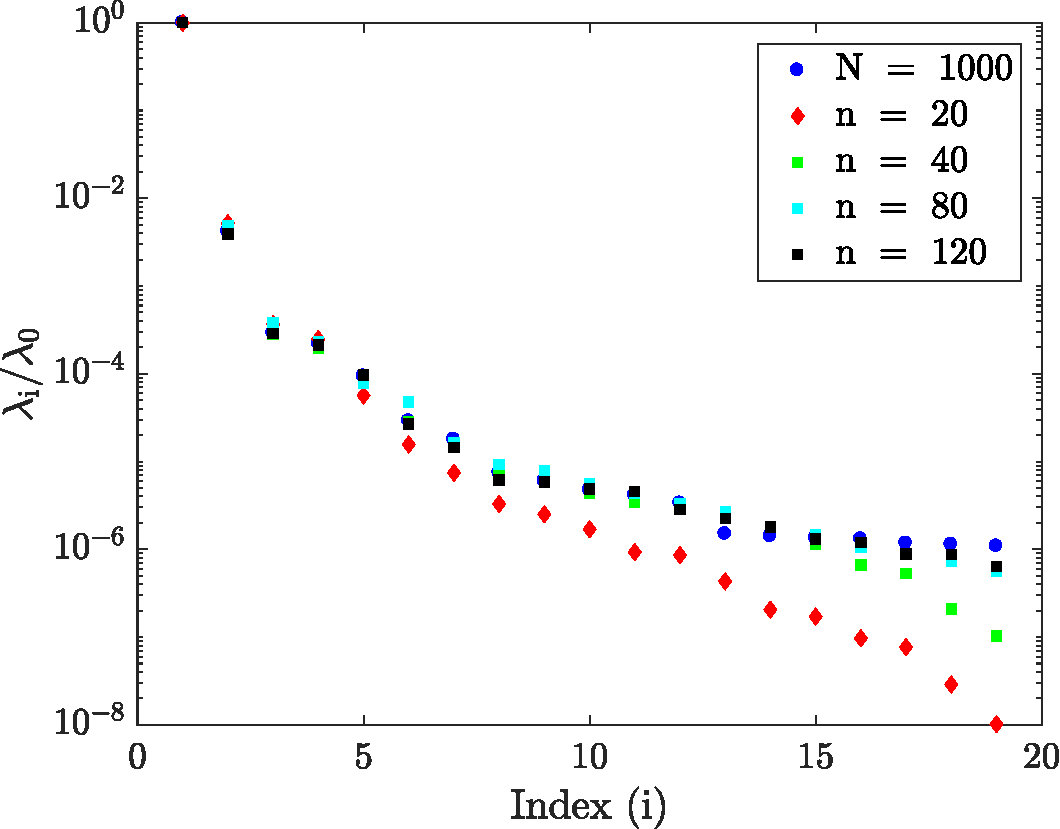
\includegraphics[width=0.45\textwidth]{./Figures/eig_comp}
   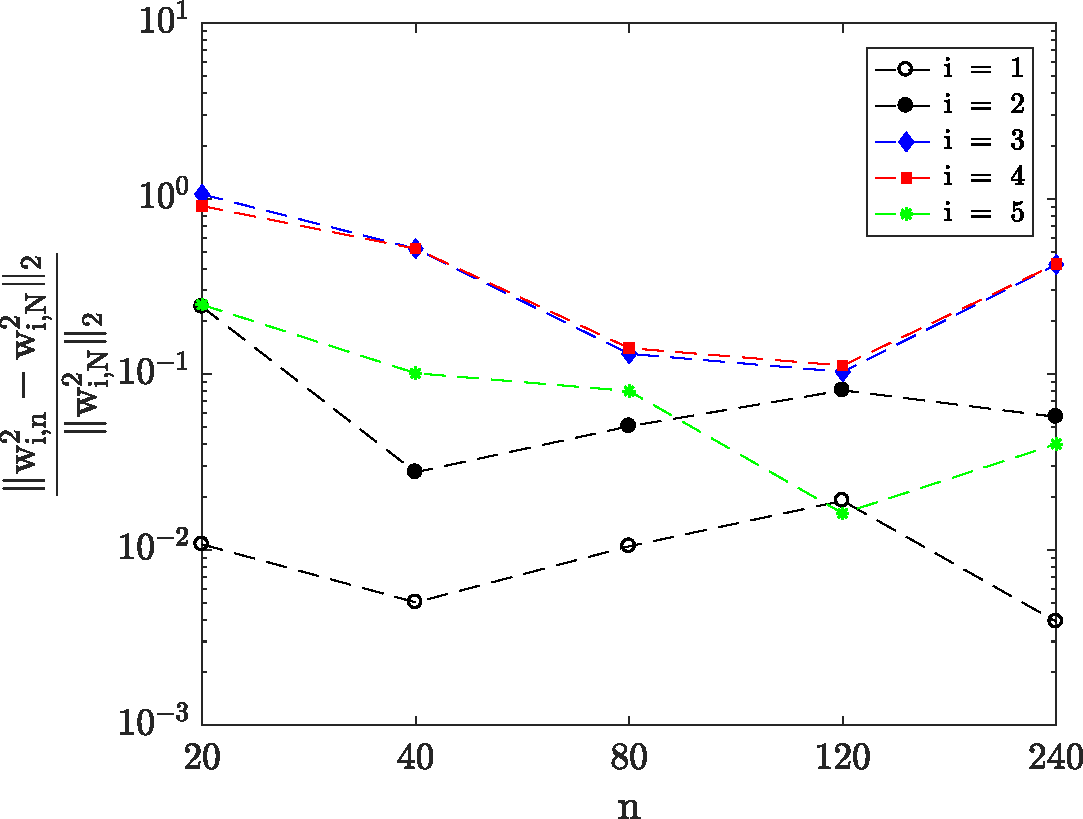
\includegraphics[width=0.48\textwidth]{./Figures/err_eigv_1_5}
\caption{Left: A comparison of the eigenvalue spectrum using $n$ = $\{20,40,80,120\}$ samples with that
obtained using a much larger sample size, $N$~=~1000. Right: Relative L-2 norm of the difference between
individual components of the first five eigenvectors of $\mat{C}$, constructed using $N$~=~1000 samples,
and using a smaller sample size, $n$ ranging from 20 to 240.} 
\label{fig:eig_comp}
\end{center}
\end{figure}
%
Interestingly, we observe that the dominant eigenvalues ($\lambda_1 - \lambda_4$) are approximated 
reasonably well with just 20 samples. As expected, the accuracy of higher-order eigenvalues is observed
to improve with the sample size. Similarly, the relative error associated with the dominant eigenvectors
($i$ = 1,2) is found to range from $\mathcal{O}(10^{-2} - 10^{-1})$ and is relatively much smaller than 
the higher-order eigenvalues. In this case, since $\left(\frac{\lambda_1}{\lambda_2}\right)\gg 1$, we have
a 1-dimensional active subspace. Hence, the first eigenvector sufficiently captures the uncertainty in
the  model output. Therefore, a sample size of 20 is adequate for computing the active subspace in this
case. The iterative strategy therefore offers a significant potential for computational advantage. 
However, estimating the gradient of the model output imposes a significant computational burden.
Hence, we explore the applicability of a so-called gradient-free approach as mentioned earlier, in the
following section.  

\subsection{Grad-free approach}
\label{sub:gradfree}

As mentioned earlier, the grad-free approach does not involve computation of the gradient of the model
output. Instead, a least-squares fit is performed to the local linear regression-based approximation
to the model output. While the grad-free approach offers a significant potential for additional 
computational savings, its ability to reasonably approximate the active subspace 
has not been investigated for a wide variety of problems~\cite{Constantine:2015}. Nevertheless, we are motivated by the
underlying potential of this approach in reducing the computational effort associated with the
active subspace computation. Moreover, this effort could help advance this approach and further motivate
its usage for a wide variety of high-dimensional applications in the future. 

First, we implement the grad-free approach to the 19-dimensional problem and compare our findings with
those obtained using the grad-based approach. Later, in
Section~\ref{sec:app}, we compute the active subspace for a 33-dimensional application using the grad-free
approach. Once again, the strategy is implemented in an iterative manner as shown in~\ref{sub:grad}. 
It is observed that the results from the grad-free approach are consistent with the grad-based approach
as discussed further below.

In the grad-free approach, the model output is first computed at an initial set of $n_1$ samples. An independent
set of $M$ samples is also drawn according to the joint probability distribution of the inputs. For each sample
in $M$, $p$ nearest neighbours in the $n_1$ set are identified. A least-squares fit to model evaluations at
the $p$ samples is performed. The slope vector ($\bm{b}_i$) of the regression-fit is stored separately and the process is
repeated for each sample in $M$. The symmetric and positive semi-definite matrix, $\hat{\mat{C}}$ is hence constructed
using the slope vectors as follows:
%
\be
\hat{\mat{C}} = \frac{1}{M}\sum\limits_{i=1}^{M}\bm{b}_i\bm{b}_i^\top = \hat{\bm{W}}\hat{\bm{\Lambda}}\hat{\bm{W}}^\top
\ee
%
Eigenvalue decomposition of $\hat{\mat{C}}$ yields an initial approximation to the
active subspace. The aforementioned sequence of steps is repeated until $\delta w_{1,j}^{(r)}$ as mentioned
earlier in~\ref{sub:grad} is found to be smaller than $\tau$. An outline of the grad-free approach is
provided in Algorithm~\ref{alg:free1}, and the specific sequence of steps pertaining to the construction of
$\hat{\mat{C}}$ is provided in Algorithm~\ref{alg:free2}.
 


\bigskip
\begin{breakablealgorithm}
\renewcommand{\algorithmicrequire}{\textbf{Input:}}
\renewcommand{\algorithmicensure}{\textbf{Output:}}
  \caption{An iterative gradient-free approach for discovering the active subspace} (\hayleynote{We can alter this the same way as we did for Algorithm 1?})
  \begin{algorithmic}[1]
\Require $\theta_l$, $\theta_u$, $M$, $\tau$. 
\Ensure $\Lambda$, $W$, $\eta$. 
    \Procedure{Gradient-free}{}
	\State Draw $n_1$ random samples, $\{\bm{\xi}_k\}_{k=1}^{n_1}$ $\in$ [-1,1]
         according to $\bm{f(\xi)}$.
	\State Project to the physical space:
        $\{\bm{\theta}_k\}_{k=1}^{n_1}=\theta_l+0.5(\theta_u-\theta_l)\{\bm{\xi}_k\}_{k=1}^{n_1}$
	\State $N_\text{total}$ = $n_1$ 
	\State Compute $G(\bm\theta_k)$, $k=1, \ldots, N_\text{total}$.
	\State Draw $M$ random samples, $\{\bm{\nu}_i\}_{i=1}^{M}$ $\in$ [-1,1]
         according to $\bm{f(\xi)}$.
	\State Construct the matrix, $\mat{C}$.
	\State Eigenvalue decomposition, $\mat{C}$ = $W^{(0)}\Lambda^{(0)} W^{(0)\top}$
	\State Partition the Eigenpairs: $\Lambda^{(0)}~=~ 
        \begin{bmatrix} \Lambda_1^{(0)} & \\ & \Lambda_2^{(0)} \end{bmatrix}$, 
        $W^{(0)}~=~\begin{bmatrix} w_1^{(0)} & w_2^{(0)} \end{bmatrix}$, 
        $\Lambda_1^{(0)}\in \mathbb{R}^{d\times\mathcal{S}}$
	\State Set $r$ = 0
	\Loop
		\State Set $r$ = $r$ + 1
		\State Draw $n_r$ = $\lceil \beta n_1 \rceil$ new random samples 
                $\{\bm{\xi}_k\}$ $\in$ [-1,1], $k = n_{r-1}+1,\ldots,n_{r-1}+n_r$.
		\State Project $\bm{\xi}_k$~$\rightarrow$~$\bm{\theta}_k$.
		\State $N_\text{total}$ = $N_\text{total}$ + $n_r$ 
		\State Compute $G(\bm\theta_k)$, $k=n_{r-1}+1, \ldots, n_{r-1}+n_r$.  
		\State Construct the matrix, $\mat{C}$.
		\State Eigenvalue decomposition, $\mat{C}$ = $W^{(r)}\Lambda^{(r)} W^{(r)\top}$
		\State Compute $\delta w_{1,j}^{(r)}$ = 
                       \scalebox{1.25}{$\frac{\|(w_{1,j}^{r})^2 - 
                       (w_{1,j}^{r-1})^2\|}{\|(w_{1,j}^{r-1})^2\|}$}, 
                       $j = 1,\ldots,\mathcal{S}$.
		\If {$\max\left(\delta w_{1,j}^{(r)}\right)<\tau$}
			\State break
		\EndIf
	\EndLoop
	\State Compute $\alpha_i(N_\text{total}) = \sum\limits_{j=1}^{\mathcal{S}} \Lambda_{1_{i,j}}w_{1_{i,j}}^2$,
	$i=1,\ldots,d$.
    \EndProcedure
  \end{algorithmic}
  \label{alg:free1}
\end{breakablealgorithm}
\bigskip

\bigskip
\begin{breakablealgorithm}
%\renewcommand{\algorithmicrequire}{\textbf{Input:}}
%\renewcommand{\algorithmicensure}{\textbf{Output:}}
  \caption{Algorithm for constructing the matrix, $\mat{C}$}
  \begin{algorithmic}[1]
	\Procedure{Local Linear Approximation}{}
	\State Draw $N$ random samples, $\{\bm{\xi}_k\}_{k=1}^{N}$ $\in$ [-1,1]
	according to $\bm{f(\xi)}$.
	\State Project to the physical space:
	$\{\bm{\theta}_k\}_{k=1}^{N}=\theta_l+0.5(\theta_u-\theta_l)\{\bm{\xi}_k\}_{k=1}^{N}$
	\State Compute $G(\bm\theta_k)$, $k=1, \ldots, N$.
	\State Draw $M$ random samples, $\{\bm{\nu}_i\}_{i=1}^{M}$ $\in$ [-1,1]
	according to $\bm{f(\xi)}$.
	\State Choose an integer $p \leq N$ 
	\State For each $i=1, \ldots, M$, compute 
	\[
	\begin{aligned}
	\Phi_i &= \{ p \text{ nearest points in } \{\bm{\xi}_k\}_{k=1}^{N} \text{ to } \bm{\nu}_i\}\\
	\vspace{-2mm}
	\Psi_i &= \text{subset of } G(\bm\theta_k) \text{ corresponding to the points in } \Phi_i
	\end{aligned}
	\]
	\State Compute linear least square fits 
	 $G(\bm\theta_k) \approx c_i + b_i^T\bm{\xi}_k$, \  $\bm{\xi}_k \in \Phi_i, \ G(\bm\theta_k) \in \Psi_i$
	\State Compute the matrix 
	\[
	\mat{C} \approx \frac{1}{M} \sum_{i=1}^{M} b_i b_i^T = {W}{\Lambda}{W}^T
	\]
	\EndProcedure
  \end{algorithmic}
  \label{alg:free2}
\end{breakablealgorithm}
\bigskip



The grad-free approach when implemented to the 19-dimensional H$_2$/O$_2$ reaction kinetics problem
with uncertain pre-exponents ($A_i$'s) also yielded a 1-dimensional active subspace. In Figure~\ref{fig:comp} (left),
we provide a comparison of the components of the dominant eigenvector, obtained using the two approaches.
Additionally, the quantity, $\delta w_{1,j}^{(r)}$ is also plotted in
Figure~\ref{fig:comp} (right) to illustrate convergence characteristics for the grad-free approach.
%
\begin{figure}[htbp]
 \begin{center}
  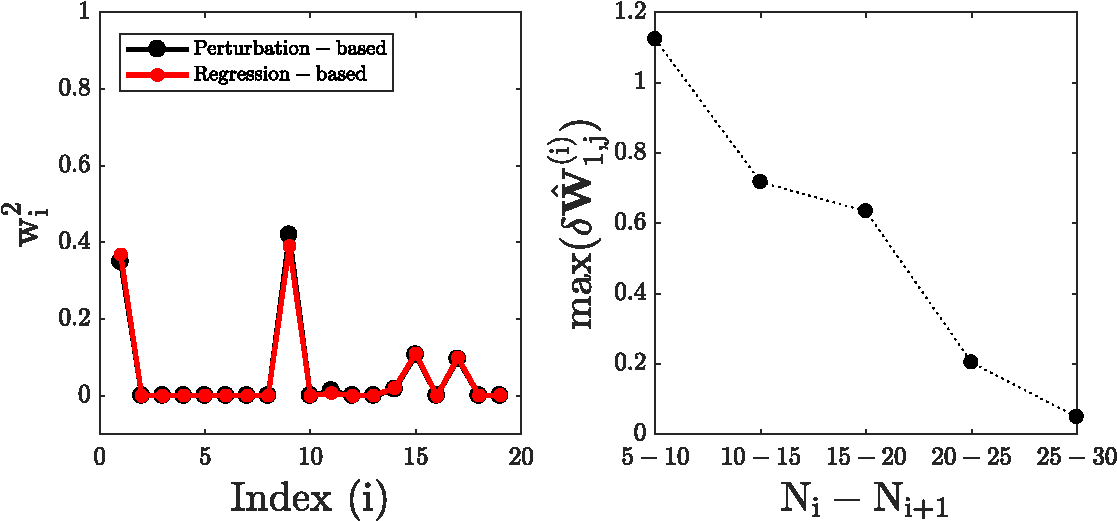
\includegraphics[width=0.8\textwidth]{./Figures/eigv6}
\caption{Left: An illustrative comparison of individual components of the converged dominant eigenvector obtained
using the two approaches discussed in~\ref{sub:grad} and~\ref{sub:gradfree}. Right: The quantity,  $\delta w_{1,j}^{(r)}$
is plotted for successive iterations to illustrate the convergence behavior.}
\label{fig:comp}
\end{center}
\end{figure}
%
Individual components of the dominant eigenvector from the two approaches are observed to be in excellent
agreement with each other. Moreover, as expected,  $\delta w_{1,j}^{(r)}$ is observed to decrease with iterations, and
the eigenvector is considered to have converged if its value is found to be smaller than 0.1. Note that only 30 samples
were found to be sufficient for approximating the active subspace in the 19-dimensional input domain. 

As mentioned earlier, the model output $f(\bm{\xi}(\bm{\theta}))$ predominantly varies in the active subspace. Hence, 
$f(\bm{\xi}(\bm{\theta}))$ can be transformed as a function of the active variable as $G(\bm{w}_1^\top\bm{\xi})$ in
the subspace. The plot of $G$ versus $\bm{w}_1^\top\bm{\xi}$, regarded as the \textit{sufficient summary plot} (SSP) is 
compared for the two approaches in Figure~\ref{fig:comp_ssp}.
%
\begin{figure}[htbp]
 \begin{center}
  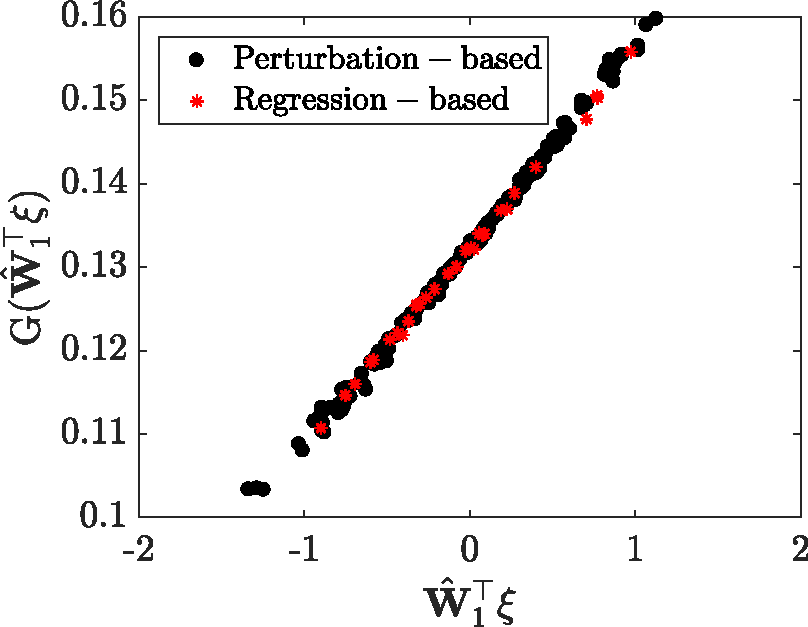
\includegraphics[width=0.48\textwidth]{./Figures/comp_ssp}
\caption{An illustrative comparison of the SSPs generated using the grad-based and the grad-free approaches.}
\label{fig:comp_ssp}
\end{center}
\end{figure}
%
The two SSPs are observed to be in excellent agreement with each other. Moreover, it is interesting to note
that the variability in ignition
delay based on the considered prior marginals for $A_i$'s is observed to be approximately linear in the
active subspace; consistent with the fact the it is 1-dimensional.

We extend the comparative assessment of the two approaches by estimating the activity score for individual
uncertain parameters ($\alpha_i$) using
the components of the dominant eigenvector in the following equation:
%
\be
\alpha_i(n) = \sum\limits_{j=1}^{\mathcal{S}}\Lambda_{1_{i,j}}w_{1_{i,j}}^2,~i = 1,\ldots,N_p
\ee
%
where $n$ is the sample size. The activity scores for the 19 uncertain pre-exponents ($A_i$'s), estimated using
the two approaches are plotted in Figure~\ref{fig:comp_as} (left). Additionally, for the purpose of verification, we 
compare these estimates with those obtained using the DGSMs~\cite{Vohra:2018} in 
Figure~\ref{fig:comp_as} (right). 
%
\begin{figure}[htbp]
 \begin{center}
  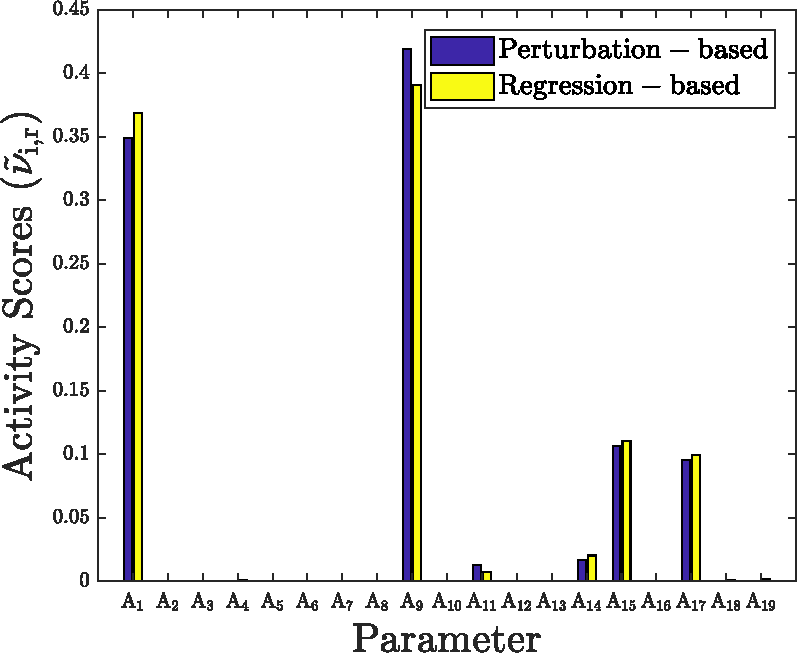
\includegraphics[width=0.45\textwidth]{./Figures/comp_as}
  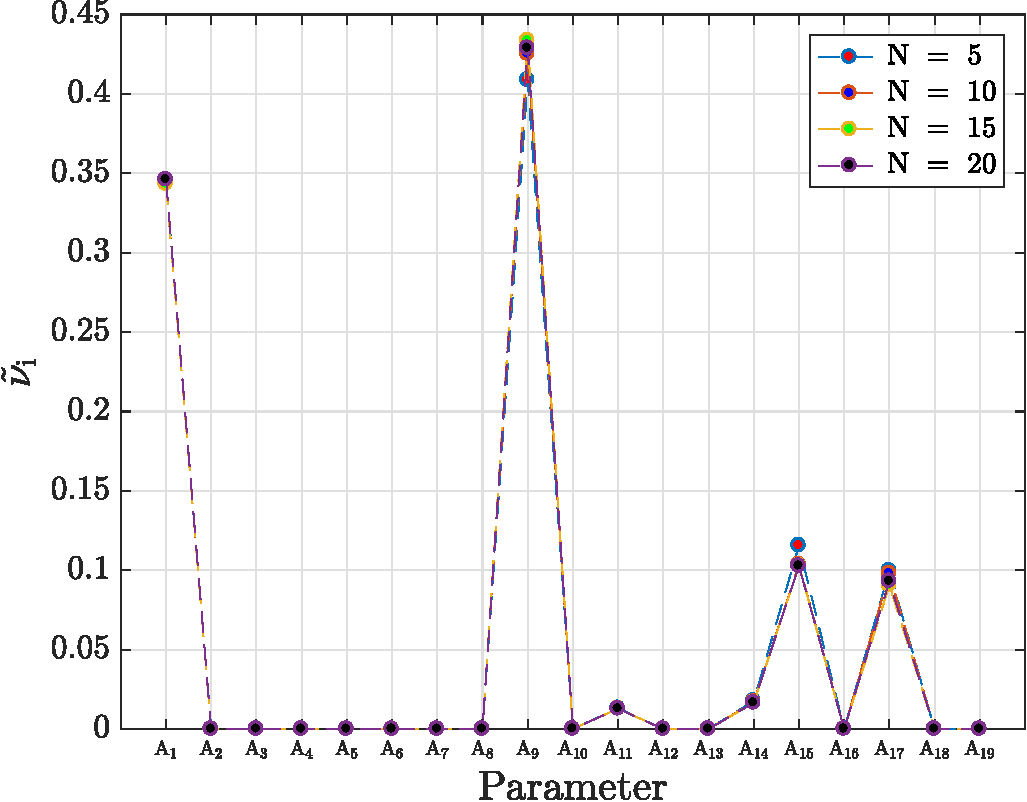
\includegraphics[width=0.45\textwidth]{./Figures/ub_conv_kinetics_rich}
\caption{Left: A bar-graph of activity scores ($\alpha_i$'s) for the 19 uncertain pre-exponents ($A_i$'s).
Right: A plot of the screening metric ($\widehat{\mathcal{C}_i\mu_i}$), defined as a normalized product of the
Poincare constant and the DGSM ($\mu_i$) (adapted from~\cite{Vohra:2018}).}
\label{fig:comp_as}
\end{center}
\end{figure}
%
The activity scores estimated using the two approaches agree favourably with each other as well as those
based on the screening metric involving the DGSMs from~\cite{Vohra:2018}. It is observed that the uncertainty
associated with the ignition delay is largely due to the uncertainty in $A_9$ and $A_1$. Sensitivity towards
$A_{15}$ and $A_{17}$ is also found to be significant. 

The above comparisons establish consistency between the two approaches. Note that the computational
effort in the case of grad-free approach is significantly smaller. Hence, we are encouraged to use the
grad-free approach for the 33-dimensional application in the next section. 



\bigskip
\bigskip
%
\section{$\text{H}_2$/$\text{O}_2$ reaction kinetics: higher-dimensional case}
\label{sec:app}

For the high-dimensional case, we aim to investigate the impact of 
uncertainty in the following problem parameters on 
the ignition delay associated with the H$_2$/O$_2$ reaction:
(i) pre-exponents ($A_i$'s); (ii) the activation energies
($E_{a,i}$'s); and (iii) the initial pressure~($P_0$),
temperature~($T_0$), and stoichiometry~($\Phi_0$). 
%
The $\log(A_i)$'s, $E_{a,i}$'s for all reactions except $\mathcal{R}_6$
-- $\mathcal{R}_9$, $\mathcal{R}_{13}$ (due to zero nominal values for $E_a$),
and the initial conditions were considered to be uniformly distributed, and
perturbed by 2$\%$ about their nominal values.
Note that the magnitude of the perturbation was selected such that the
ignition delay assumes a physically meaningful value in the input domain. 
The nominal values of the rate parameters, $A_i$'s and $E_{a,i}$'s 
were taken from~\cite{Yetter:1991}. The nominal values of $P_0$, $T_0$, and
$\Phi_0$ were considered to be 1.0~atm, 900~K, and 2.0 respectively.

\subsection{Computing the active subspace}

The active subspace was computed using the iterative procedure outlined in 
Algorithm~\ref{alg:grad}. The convergence of the eigenvectors was examined
by tracking the quantity `$\rebut{\max\limits_j}(\delta \hat{\mat{W}}_{1,j}^{(i)})$'. 
In Figure~\ref{fig:conv_app}~(right), we examine $\rebut{\max\limits_j}(\delta \hat{\mat{W}}_{1,j}^{(i)})$
with increasing iterations for the perturbation and the regression approaches 
discussed earlier in Section~\ref{sec:method}. 
%
\begin{figure}[htbp]
 \begin{center}
  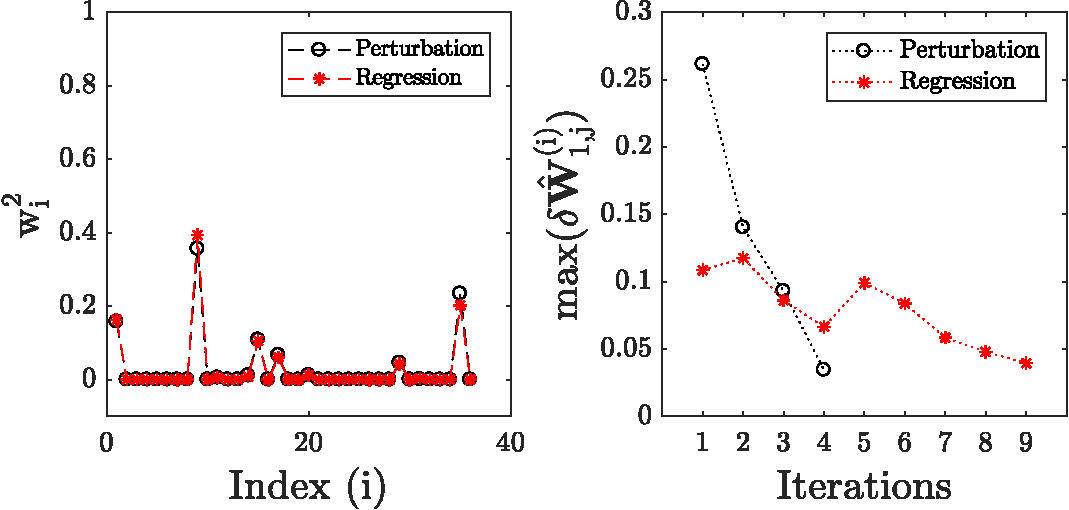
\includegraphics[width=0.8\textwidth]{./Figures/eig_conv36Dp2}
\caption{Left: An illustrative comparison of individual components of the 
dominant eigenvector in the converged active subspace i.e., at the end
of 4 iterations in the perturbation approach and 9 iterations in the
regression approach. Right: A comparison of the convergence behavior
of the perturbation and the
regression approaches. Convergence is accomplished once 
$\rebut{\max\limits_j}(\delta \hat{\mat{W}}_{1,j}^{(i)})$ assumes a value smaller
than 0.05.}
\label{fig:conv_app}
\end{center}
\end{figure}
%
At each iteration, we improve our estimates of the matrix $\hat{\mat{C}}$ by
estimating the gradient of the ignition delay at 5 new randomly generated samples 
in the 36-dimensional input space. However, gradient computation at these
5 samples requires 185 (=5$\times$(36+1)) model runs when using perturbation. 
For the same computational effort, the regression approach can afford 185 new
samples at each iteration. It is observed that using $\tau$ = 0.05, the 
active subspace requires 4 iterations (925 model runs) to converge in the case of perturbation, and
9 iterations (1850 model runs) to converge in the case of regression. Hence, the computational effort
required to obtain a converged active subspace is doubled when using
regression to approximate the gradient. Moreover, gradient estimation in the perturbation approach
can be made more efficient by using techniques such as automatic differentiation~\cite{Kiparissides:2009}
and adjoint computation~\cite{Jameson:1988}. These techniques although not pursued here are 
promising directions for
future efforts pertaining to this work. In Figure~\ref{fig:conv_app}~(right), we compare
individual components of the dominant eigenvector in the converged active subspace
obtained using the two approaches. The components are observed to be in excellent
agreement with each other.

In Figure~\ref{fig:hd}, we plot the SSP for the perturbation approach (left) and the regression
approach (center) in a 1-dimensional active subspace. A 1-dimensional polynomial fit is also
illustrated in both cases. Moreover, the two surrogates are shown to be consistent with each other (right).
From these results, it is clear that a 1-dimensional active subspace captures the variability in the
ignition delay with reasonable accuracy, and that the two approaches yield consistent results.
%
\begin{figure}[htbp]
 \begin{center}
   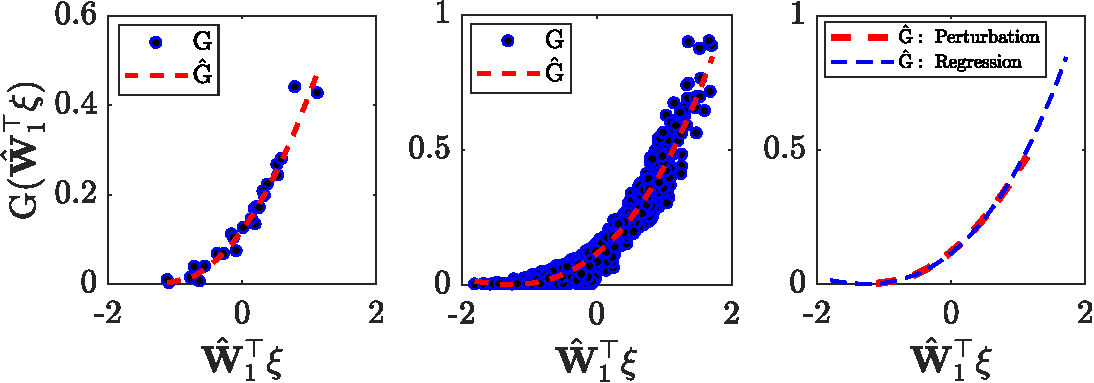
\includegraphics[width=0.9\textwidth]{./Figures/SSP_plot36Dp2}
\caption{Sufficient summary plots (SSPs) for the case of perturbation (left) and regression (center).
A polynomial fit of degree 2 and 3 as shown in the plots is used as a surrogate in the 
perturbation and regression approaches respectively. An illustrative comparison of the two
surrogates is also provided (right).}
\label{fig:hd}
\end{center}
\end{figure}
%

\subsection{Surrogate Assessment}
\label{sub:verify}

The 1-dimensional surrogate ($\hat{G}$) shown in Figure~\ref{fig:hd} for the perturbation
and regression approaches is investigated for its ability to capture the uncertainty in the
ignition delay. Specifically, we compare probability density functions (PDFs)
obtained using the true set of model evaluations, and 1-dimensional
surrogates ($\hat{G}$'s) based on the two approaches, as shown in 
Figure~\ref{fig:pdf_36D}. Note that the three PDFs were evaluated using the same set of 10$^4$ samples in the 
cross-validation set. 
%
\begin{figure}[htbp]
\begin{center}
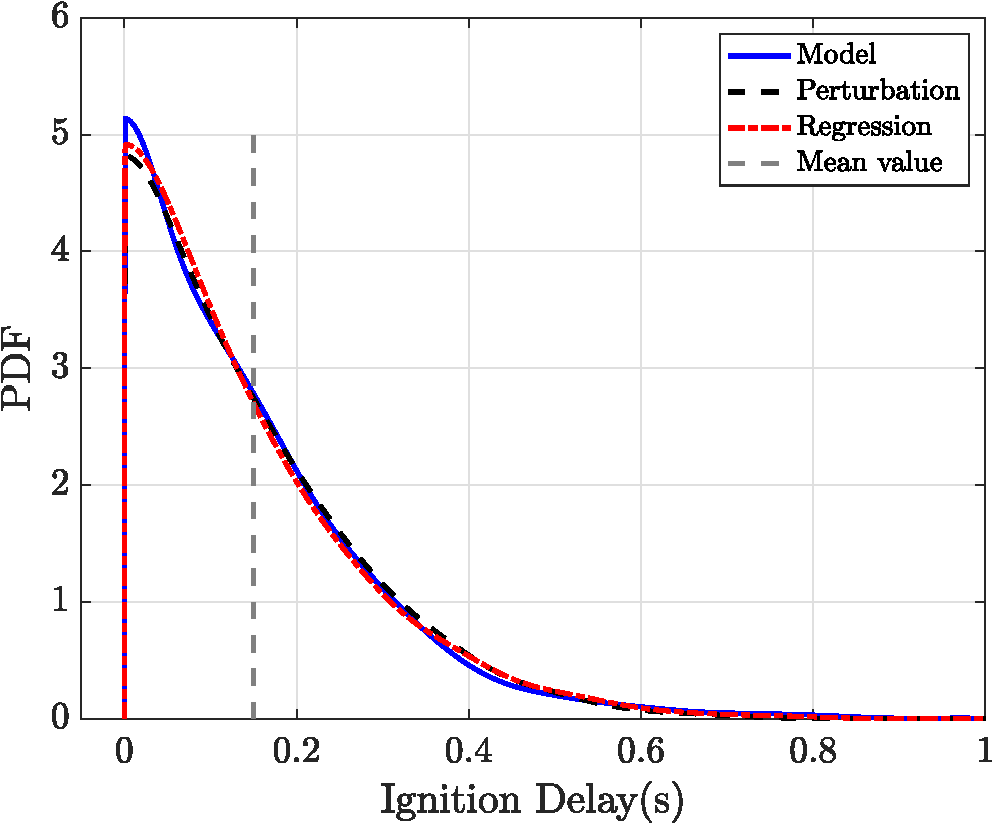
\includegraphics[width=3.0in]{./Figures/pdf_plot36Dp2}
\end{center} 
\caption{A comparison of the PDFs of ignition delay, obtained using model 
evaluations (solid line) and 1-dimensional surrogates using the regression-based strategy (dashed line) and the
perturbation-based strategy (dashed-dotted line). The same set of 10$^4$ samples in the cross-validation set were 
used in each case.}
\label{fig:pdf_36D}
\end{figure}
%
The PDFs are observed to be in close agreement with each other. Specifically, the modal
estimate and the uncertainty (quantified by the spread in the distributions) is found to be consistent for the three 
cases. To confirm this, we further compute the first-order (mean) and the second-order (standard deviation) 
statistics
of the estimates of the ignition delay obtained using the model, 1-dimensional surrogate from perturbation, and
1-dimensional surrogate from regression at the cross-validation sample set. The mean and standard deviation
estimates are provided in Table~\ref{tab:stats}.
%
\begin{table}[htbp]
\begin{center}
\begin{tabular}{ccc}
\toprule
$\textbf{Distribution}$ & $\mu$ & $\sigma$ \\ 
\bottomrule
$G$~(Model) & \rebut{0.15} & \rebut{0.14} \\
$\hat{G}$~(Perturbation-based) & \rebut{0.15} & \rebut{0.13} \\
$\hat{G}$~(Regression-based) & \rebut{0.15} & \rebut{0.13} \\
\bottomrule
\end{tabular}
\caption{The mean ($\mu$), and the standard deviation ($\sigma$), computed using the model ($G$), and
the surrogate ($\hat{G}$) based on the two strategies at 10$^4$ samples in the cross-validation
set.}
\label{tab:stats}
\end{center}
\end{table}
%
The mean and the standard deviation estimates obtained using the model and the 1-dimensional surrogates
are found to be in close agreement. Hence, the uncertainty in the ignition delay is accurately captured 
in both cases.

\subsection{GSA consistency check}

The normalized activity scores ($\tilde{\nu}_{i,r}$) based on the 1-dimensional active subspace, obtained
using the two approaches for gradient estimation (perturbation and regression),
are compared with the 
total-effect Sobol' indices
in Figure~\ref{fig:as_36D}. Note that the Sobol' indices were computed using the verified
1-dimensional surrogate ($\hat{G}$) in the active subspace, obtained using the 
perturbation approach. 
%
\begin{figure}[htbp]
 \begin{center}
  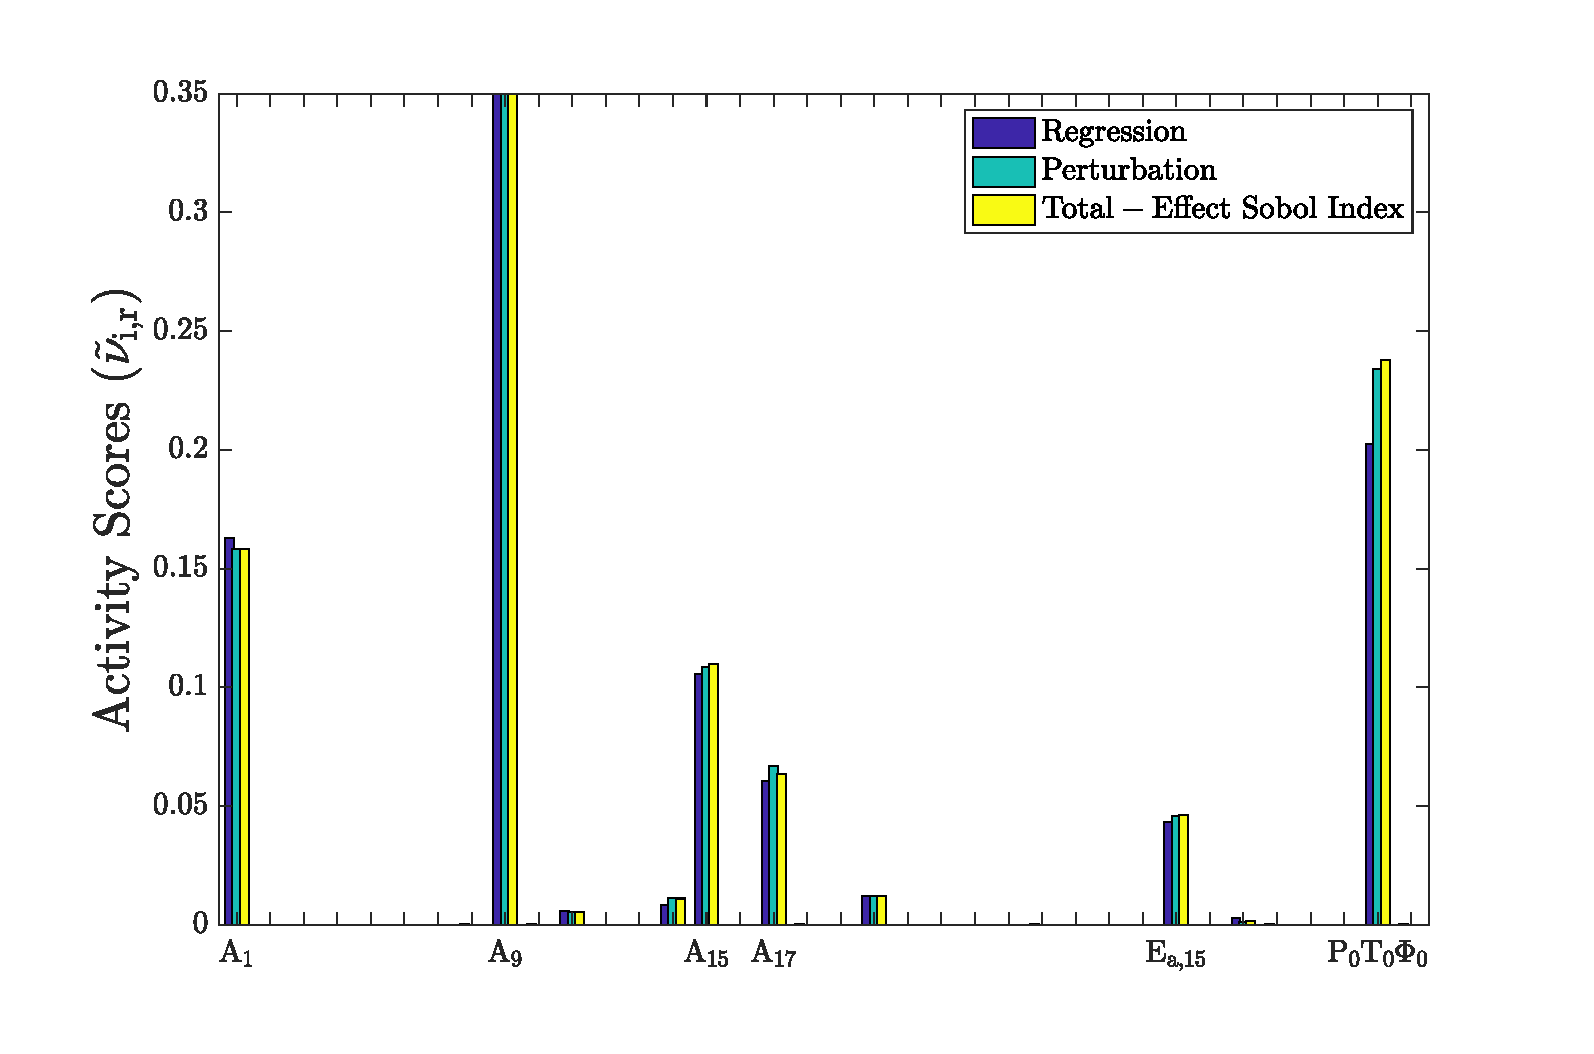
\includegraphics[width=0.8\textwidth]{./Figures/as_36Dp2_rev2}
\caption{Bar graphs illustrating individual activity scores for the uncertain 
rate parameters and the initial conditions for the H$_2$/O$_2$ reaction.}
\label{fig:as_36D}
\end{center}
\end{figure}
%
Several useful inferences can be drawn. Firstly, the normalized activity scores from the two approaches
and the total-effect Sobol' indices are found to be in close agreement with each other. Secondly, as expected, 
$\tilde{\nu}_{i,r}$ based on perturbation exhibits a better agreement with the total-effect Sobol' indices since
the 1-dimensional
surrogate based on the same approach was used to evaluate the Sobol' indices. This observation demonstrates
that the proposed framework is self-consistent. Thirdly, the variability in the ignition delay is predominantly due
to the uncertainty in $A_1$, $A_9$, and $T_0$ while contributions from the uncertainty in $A_{15}$, $A_{17}$, and
$E_{a,15}$, and $T_0$ are also found to be significant. The remaining rate parameters, initial pressure ($P_0$),
and  stoichiometry ($\Phi_0$) do not seem to impact the ignition delay in their considered intervals. 
Therefore, GSA has helped
identify the important rate parameters i.e. key contributors to the uncertainty, and also demonstrated that among the 
considered uncertain initial conditions, the ignition delay is mainly impacted by the perturbations in the initial 
temperature in the considered interval.

\rebut{As shown in the PDF plotted in Figure~\ref{fig:pdf_36D}, the ignition delay assumes a wide range of values, i.e.
from about 2~ms to 400~ms. However, for many practical applications, a much smaller ignition delay (0.1~ms--1~ms) might
be of interest. The authors would like to point out that the proposed framework was also implemented to such a regime
by using a nominal value of the initial temperature, $T_0$ = 1000~K, and the initial pressure, $P_0$ = 1.5~atm. 
Our analysis for this
regime once again revealed that a 1-dimensional active subspace was able to capture the variability in the ingition delay due to
the uncertainty in the rate-controlling parameters and the input conditions. The sensitivity trends were also found to
be qualitatively similar to those presented in Figure~\ref{fig:as_36D}. We have not included these results in the interest
of brevity. Therefore, the proposed methodology was tested
for is robustness and applicability for a wide range of conditions pertaining to the considered application.}  

\bigskip
\bigskip

\section{Summary and Discussion}
\label{sec:conc}
 
In this work, we focused on the uncertainty associated with the
rate-controlling parameters in the H$_2$/O$_2$ reaction mechanism
\rebut{as well as the initial pressure, temperature, and stoichiometry} and its
impact on ignition delay predictions. The mechanism involves 19 different
reactions and in each case, the reaction rate depends upon the choice of a
pre-exponent and an activation energy. Hence, in theory, the evolution of the
chemical system depends upon 38 rate parameters \rebut{and three initial conditions}.
However, we considered 
epistemic uncertainty in all pre-exponents and activation energies with non-zero
nominal values i.e. a total of 33 rate parameters instead of 38 \rebut{in addition to
the three initial conditions}.  
%Conventional means for uncertainty quantification such as those involving
%surrogate model construction as well as sensitivity analysis would thus be
%computationally challenging.
To facilitate efficient uncertainty analysis, we focused our efforts on
reducing the dimensionality of the problem by identifying important directions
in the parameter space such that the model output 
predominantly varies along these directions. These important directions
constitute the active subspace. Additionally, we demonstrated that the activity scores,
computed using the components of the dominant eigenvectors provide an efficient
means for approximating derivative based global sensitivity measures (DGSMs).
Furthermore, we established generalized mathematical linkages between the
different global sensitivity measures: activity scores, DGSMs, and total Sobol'
index which could be exploited to reduce computational effort associated with
global sensitivity analysis. 
 
Active subspace computation requires repeated evaluations of the gradient of
the QoI i.e. the ignition delay. For this purpose, we explored two approaches,
namely, perturbation and regression. Both approaches were shown to yield
consistent results for the 19-dimensional problem wherein only the
pre-exponents were considered to be uncertain.  \rebut{It was observed that the
computational effort required to obtain a converged active subspace was
comparable for the two approaches. However, the predictive accuracy of the
perturbation approach was found to be relatively higher. Moreover, a
1-dimensional active subspace was shown to reasonably approximate the
uncertainty in the ignition delay.} Additionally, the activity scores were also
shown to be consistent with the screening metric estimates based on DGSMs
in~\cite{Vohra:2018}. An iterative procedure was adopted to enhance the
computational efficiency. 

The active subspace was further computed for a 36-dimensional problem
wherein all pre-exponents and activation energies with non-zero nominal
estimates \rebut{as well as the initial conditions} were considered uncertain. 
\rebut{Once again, consistent results were obtained using the two approaches.
A 1-dimensional active subspace was shown to reasonably
capture the uncertainty in the ignition delay in this case. However, the
computational effort required to compute a converged active subspace
using perturbation was found to be half of the effort required in the case
of regression. Predictive accuracy of the two approaches was found to 
be comparable. Hence, perturbation seems like a preferred approach
for the higher-dimensional problem based on our findings. GSA results indicated
that the variability in the ignition delay is predominantly due to the 
uncertainty in the rate parameters, $A_1$ and $A_9$ with significant
contributions from $A_{15}$, $A_{17}$, and $E_{a,15}$. Additionally, the
ignition delay was found to be sensitive towards $T_0$.}

Based on our findings, the perturbation approach is preferable for active
subspace computation; moreover, this can be made extremely efficient, when more
efficient gradient computation techniques (adjoints-based, automatic
differentiation, etc.) are feasible. The regression-based approach can be
explored in situations involving intensive simulations where gradient
computation is very challenging. 

%
%and the goal is obtaining rough estimates of the statistics of the QoI as
%opposed to a more detailed analysis such as those involving parametric
%sensitivity.  
%
We also mention that alternate regression based approaches such as ones based
on computing a global quadratic model have been proposed and used in the
literature; see e.g.,~\cite{Constantine:2017a}.  The applicability of such an
approach in the context of high-dimensional chemical reaction networks is
subject to future work. 

The computational framework presented in this work is agnostic to the choice of
the chemical system and can be easily adapted for other systems as long as the
quantity of interest is continuously differentiable in the considered domain of
the inputs.  We have demonstrated that the active subspace could be exploited
for efficient forward propagation of the uncertainty from inputs to the output.
The resulting activity scores and the low-dimensional surrogate could further
guide optimal allocation of computational resources for calibration of the
important rate-controlling parameters \rebut{and input conditions} in a
Bayesian setting.  Additionally, dimension reduction using active subspaces
could assist in developing robust formulations for predicting discrepancy
between simulations and measurements due to epistemic uncertainty in the model
inputs.

\bigskip
\bigskip

\section*{Acknowledgment}

M. Vohra and S. Mahadevan gratefully acknowledge funding support from the
National Science Foundation (Grant No. 1404823, CDSE Program), and Sandia
National Laboratories (PO No. 1643376, Technical monitor: Dr. Joshua Mullins).
The authors also thank Dr.~Cosmin Safta at Sandia National
Laboratories for his guidance pertaining to the usage of the TChem software\
package.

\bigskip
\bigskip

\bibliographystyle{elsarticle-num}
%\bibliographystyle{unsrt}
\bibliography{REFER}

\end{document}
